\chapter{Design and solution}
\section{Gathering data}
% TODO: Thu thập dữ liệu và phân loại như thế nào -> Lấy từ web ..., các video thủ ngữ trên zootube
% TODO: Tiến hành tổng hợp và phân loại -> tổng hợp thành bảng, phần loại từ thành các pattern, location, direction để chuẩn bị cho mấy mục dưới
% TODO: Chèn hình về cái sheet vào



Before we can design a system that can translate sign language, we must first understand what a sign language word is and where to collect the data. After observing the sign language on the websites \url{https://tudienngonngukyhieu.com/} and \url{https://qipedc.moet.gov.vn/}, we noticed that some of the words have the same pattern. Furthermore, the sign's meaning is determined by its orientation and location. Furthermore, some of the terms require hand or finger movements to represent the meaning. As a result, using those four factors, we can convert a word from sign language to Vietnamese.

However, we must first collect sign language data for the thesis's model training phase. Fortunately, those two websites contain a sufficient number of sign language words. We also learned a few words from YouTube videos taught by Mrs. Le Thi Thu Xuong\cite{yt:LeThiThuXuong} and channel CDS, Central Deaf Services in Dang Nang, Vietnam\cite{yt:CDS}. As a result, we can independently train and test our system.

We gathered a large number of words from those two websites and YouTube channel to prepare the data. Then we label and divide it into many elements, which we will discuss later in the Section \ref{sec:handstate}. For the data we collected, we created a Google Sheet. We have prepared many labeled words in this file (see Figure \ref{fig:Chap4-Label-Word}). In addition, we have a sheet for many different hand shapes (see Figure \ref{fig:Chap4-Sheet-Pattern}), which helps us classify hand patterns.

\begin{figure}[H]
	\centering
	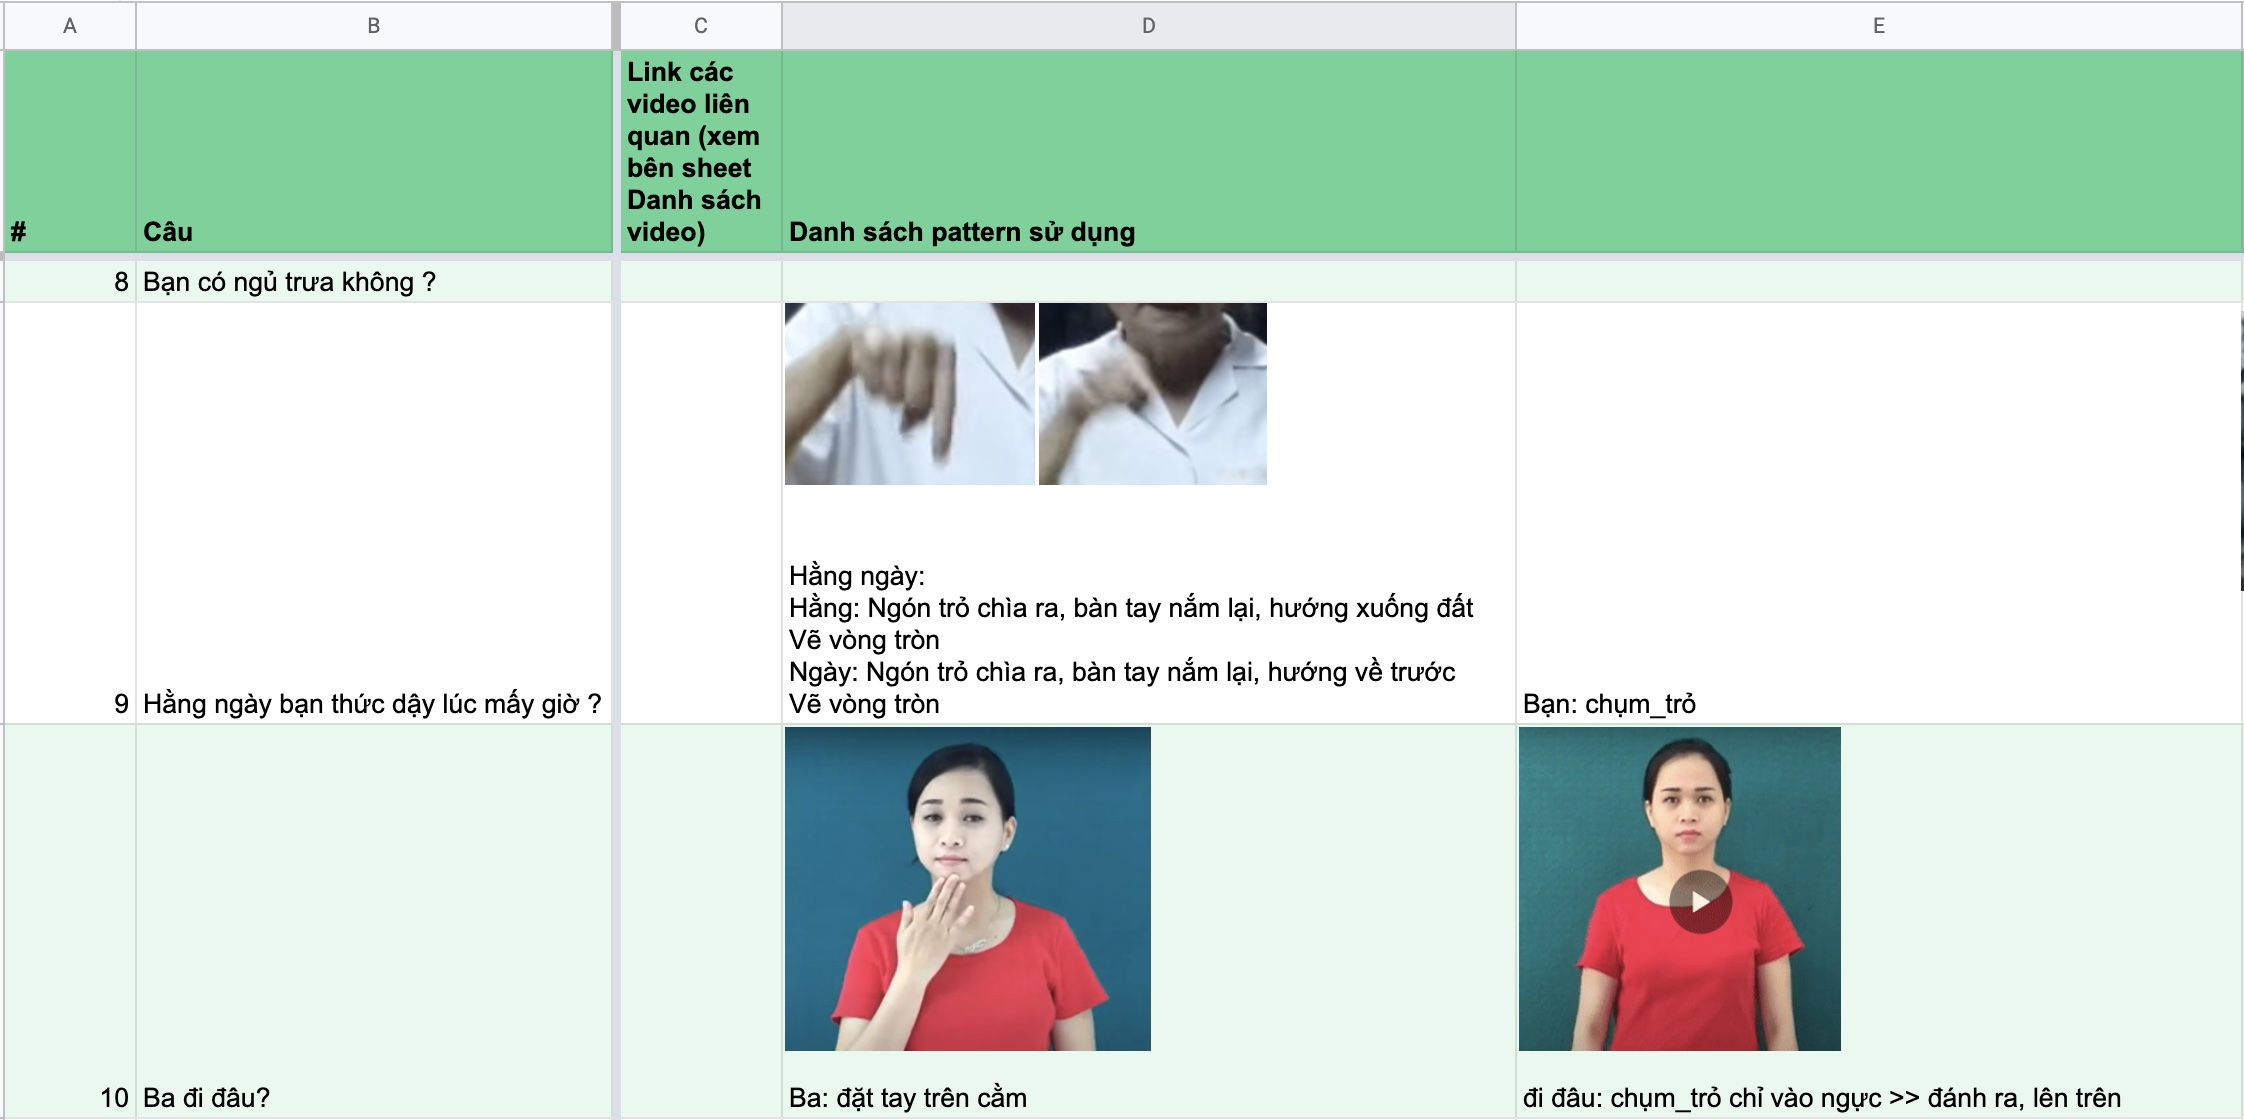
\includegraphics[width=0.9\textwidth]{img/Chap4/Label-Word.jpg}
	\caption{Google sheet about words labeled}
	\label{fig:Chap4-Label-Word}
\end{figure}

\begin{figure}[H]
	\centering
	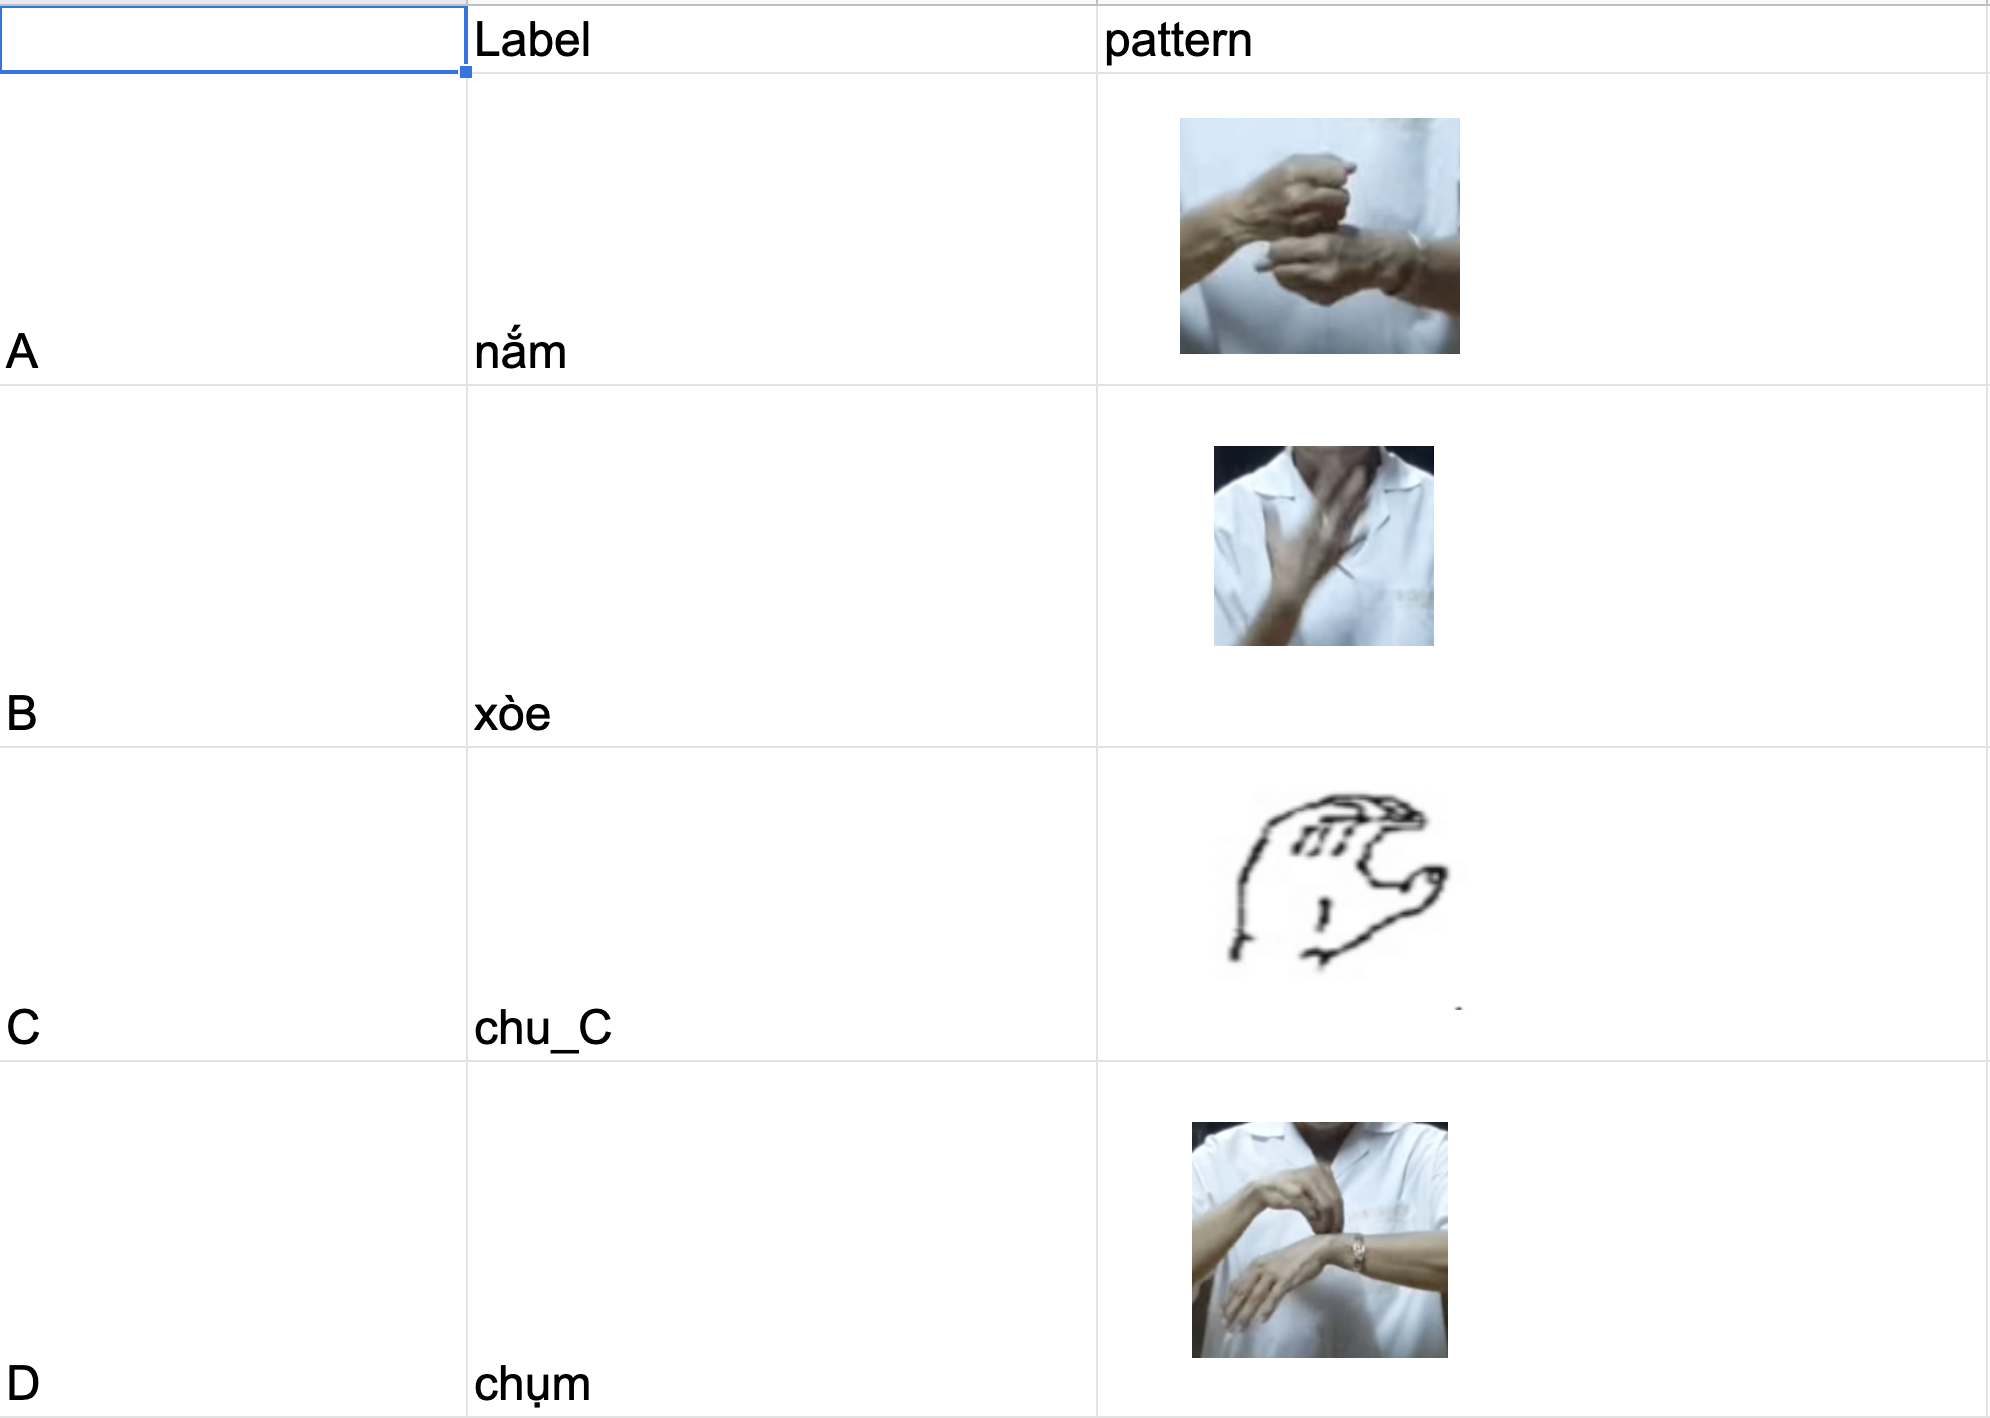
\includegraphics[width=0.9\textwidth]{img/Chap4/Sheet-Pattern.png}
	\caption{Google sheet about hand shapes can be recognized}
	\label{fig:Chap4-Sheet-Pattern}
\end{figure}



\section{System structure}

Overall, the system is composed of three hardware modules: a camera module, the user's smartphone, and the server. The server, which will be the focus of this thesis, is one of those modules that handles the most complex work.

Our artificial intelligence system for sign language translation consists of six major modules: hand pattern recognition, direction determination, location detection, action detection, word decoder, and text to speech (Figure \ref{fig:Chap4-OverviewOfTheSystemModules-Old}). To begin, the system continuously captures the motion of the hand, processes it with the hand landmark model, and then stores it in those modules. Each of them plays a distinct role. The word decoder module will take the output data and produce the corresponding outcome after combining the results of the first four modules (hand pattern, direction, location, and action detection). The result will then appear on the main screen, while the phone will speak out that word.

\begin{figure}[H]
	\centering
	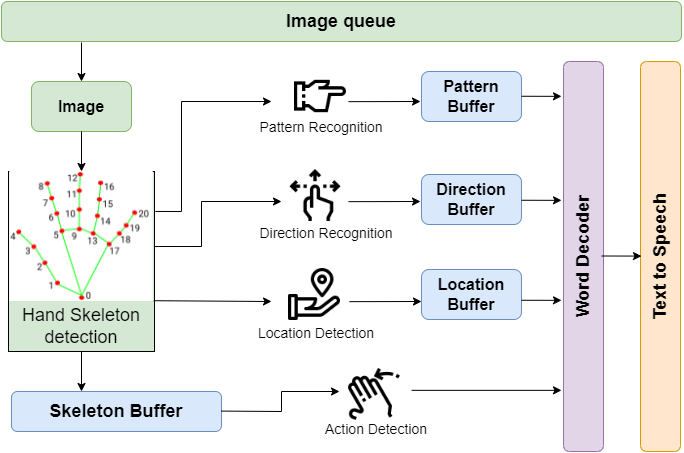
\includegraphics[width=0.9\textwidth]{img/Chap4/OverviewOfTheSystemModules-Old.png}
	\caption{Overview of the old system structure}
	\label{fig:Chap4-OverviewOfTheSystemModules-Old}
\end{figure}

Those six major modules mentioned above are the ones we had planned for at the start of the thesis. Despite going through most of the modules, we found it difficult to build the action detection module during the implementation period. It is problematic because of the demands it places on the smartphone and server.

There are some sign language words that contain a lot of moving patterns. The first method is to send the entire video captured by the camera to the server for processing. This method, on the other hand, necessitates a strong connection between the camera module, smartphone, and server and places strain on the physical devices (the camera and smartphone); as a result, those devices will become hot and may be damaged in some way. Another option is to increase the frame rate to get the action, but this can put the devices under strain. Furthermore, we must have an algorithm that is constantly processing and detecting movements, which we admit is difficult to achieve.
To solve the problem, we had to deprecate that module and change our method for obtaining the correct Vietnamese word. Instead of combining the four modules, including the action detection module, there are now only three remaining: pattern, direction, and location. Furthermore, in the word decoder module, we use the beam search heuristic search algorithm, which uses the results of the three modules to look up the word in the database and return it to us. Section \ref{sec:DetailImplementation} will go over each module's role and how it works.

\begin{figure}[H]
	\centering
	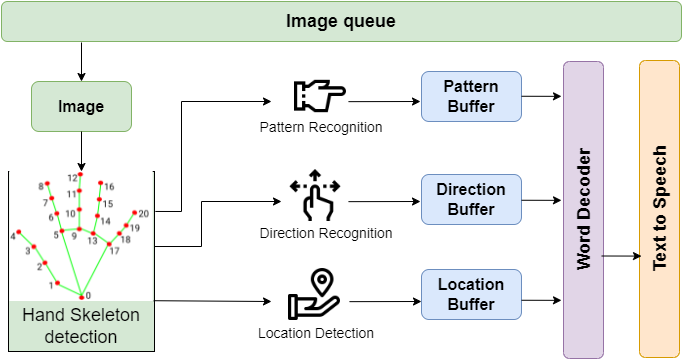
\includegraphics[width=0.9\textwidth]{img/Chap4/OverviewOfTheSystemModules-New.png}
	\caption{Overview of the new system structure}
	\label{fig:Chap4-OverviewOfTheSystemModules-New}
\end{figure}

\section{Detail implementation}\label{sec:DetailImplementation}

\subsection{Hand pattern recognition}

The first and most fundamental module of this system is hand pattern recognition. When a person with a disability performs sign language, their hands move in a variety of ways, with their hands spread out, clenched, or their fingers pointing out at something. As a result, the role of this module is to recognize the hand pattern. The system can then provide the final result by combining the outcome with other modules.

This module makes use of the hand landmark model's output, which has a matrix size of 21. We get a new matrix representing the distance between those 21 coordinates after calculating all of the values in that matrix. As seen in Figure \ref{fig:Chap4-OverviewOfTheSystemModules-New}, using the distance matrix as the input of CNN with the designed structure (see Figure \ref{fig:Chap4-StructureOfConvolutionalNeuralNetwork}) will tell us the pattern of the hand at the time it is captured.

\begin{figure}[H]
	\centering
	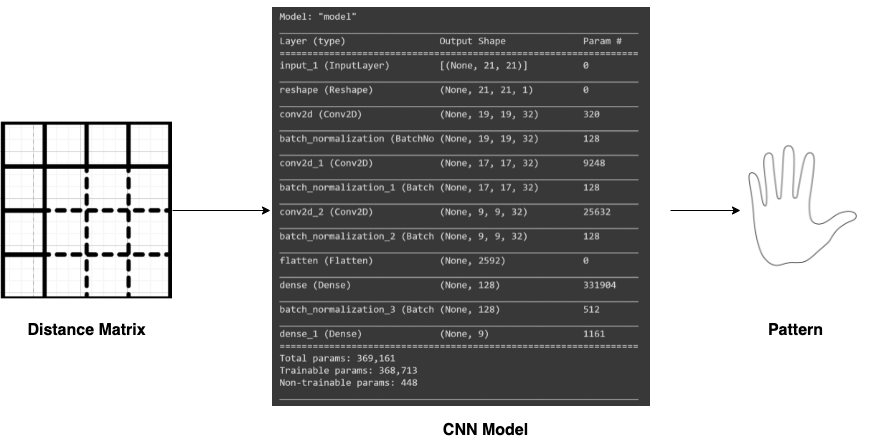
\includegraphics[width=\textwidth]{img/Chap4/Hand-Pattern-Reg-Model.png}
	\caption{Hand pattern recognition pipe line}
	\label{fig:Chap4-StructureOfConvolutionalNeuralNetwork}
\end{figure}

\subsection{Direction determination}

The hand has four directions, which are right, left, up, down, front, and back. The pattern of each hand, when combined with different directions, yields a different meaning. For example, the pattern that points at someone means the word "you," whereas the pattern that points at ourselves means the word "I." (see Figure \ref{fig:Chap4-WordYouInSignLanguage} and Figure \ref{fig:Chap4-WordIInSignLanguage}).

\begin{figure}[H]
	\centering
	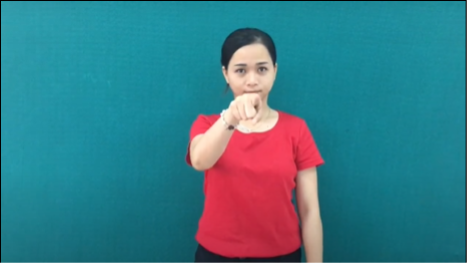
\includegraphics[width=0.6\textwidth]{img/Chap4/WordYouInSignLanguage.png}
	\caption{Word "You" (bạn) in sign language}
	\label{fig:Chap4-WordYouInSignLanguage}
\end{figure}

\begin{figure}[H]
	\centering
	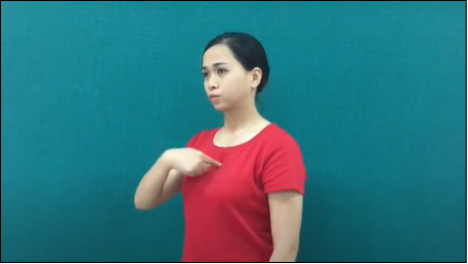
\includegraphics[width=0.6\textwidth]{img/Chap4/WordIInSignLanguage.png}
	\caption{Word "I" (tôi) in sign language}
	\label{fig:Chap4-WordIInSignLanguage}
\end{figure}

We use the hand landmark model provided by MediaPipe to determine the direction of the hand (see Section \ref{sec:MediaPipe}). The idea here is to calculate the distance between the tip of the index finger and the wrist, which is known as a \textbf{vector(0, 8)}, and then project it to the axes Ox, Oy, and Oz, in that order. Following that, we compare those coordinates to the others. Finally, the one of immense value will tell us which axis the hand is on; additionally, we will know which direction the hand is by projecting the direction from the wrist to the tip of the index finger on that corresponding axis.

\begin{figure}[H]
	\centering
	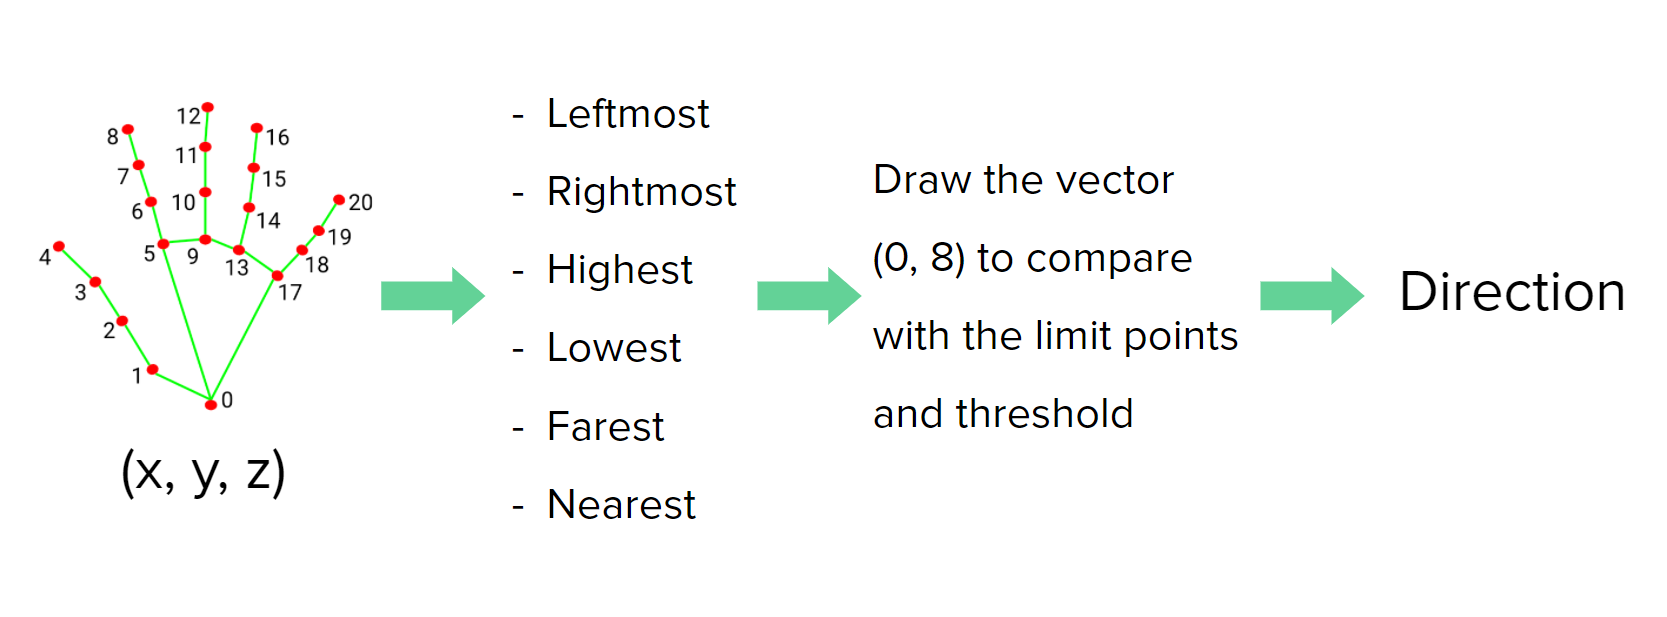
\includegraphics[width=\textwidth]{img/Chap4/DirectionSteps.png}
	\caption{Steps to detect the direction of the hand}
	\label{fig:Chap4-DirectionSteps}
\end{figure}

For instance, a hand is pointing in the left direction. When projected on the axis Ox, the distance value will be the largest of the three projected values. Then, compute the vector drawn from the wrist to the tip of the index finger; we'll know the hand's direction.

\begin{figure}[H]
	\centering
	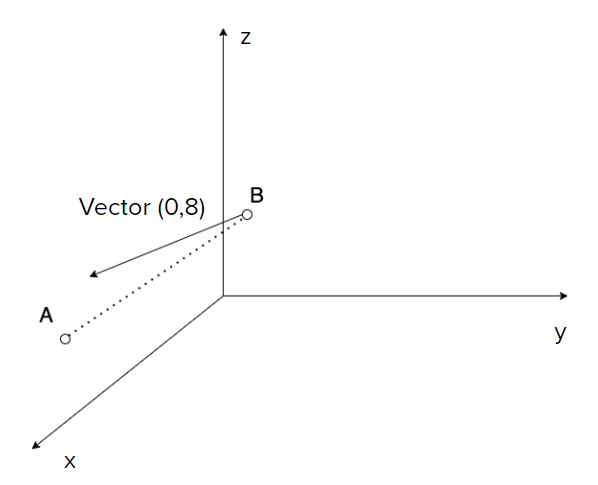
\includegraphics[width=0.6\textwidth]{img/Chap4/vector0-8-forwardLeft.png}
	\caption{Vector(0, 8) represent the hand pointing toward the left}
	\label{fig:Chap4-vector0-8-forwardLeft}
\end{figure}

\subsection{Location detection}\label{sec:locationDetection}

Hand placement differs; is the hand on the brow, mouth, or chest level, and so on. Each hand pattern associated with each location will yield a different set of words. Nonetheless, with only one camera and a view from above, it is difficult for the AI to determine the coordinates of the hand (see Figure \ref{fig:Chap4-ViewFromCamera}). However, we devised some solutions to this problem.

% The first method we use to determine the location of the hand is zooming. In this solution, we will take images of hands and calculate their size in each frame to determine whether those hands are growing or shrinking. As a result, if those hands are smaller than before, they are getting further away from the camera, and their locations are somewhere near the chest or stomach. Otherwise, the hand is closer to the camera, at the level of the mouth, nose, or forehead.

\begin{figure}[H]
	\centering
	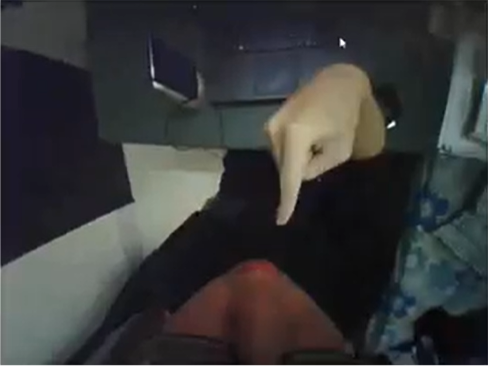
\includegraphics[width=0.6\textwidth]{img/Chap4/ViewFromCamera.png}
	\caption{View from the camera module}
	\label{fig:Chap4-ViewFromCamera}
\end{figure}

% Nonetheless, the above solution has a flaw: each man's hand is different in size, and the system does not know the correct hand position. Another option is to use a wide-angle camera that is positioned away from the brow. The camera can have a much wider field of view with this solution. Nonetheless, because we only had a standard-angle camera, we couldn't test this solution and confirm its suitability.

The first solution to detect the hand's location is using an ultrasonic sensor. In short, this sensor is an instrument that measures the distance to an object using ultrasonic sound waves (see Figure \ref{fig:Chap4-UltrasonicSensorFunction}). It works by emitting a sound wave with a frequency above the human hearing range. The sensor's transducer functions as a microphone, receiving and transmitting ultrasonic sound. The sensor measures the time between sending and receiving an ultrasonic pulse to determine the distance to a target.

\begin{figure}[H]
	\centering
	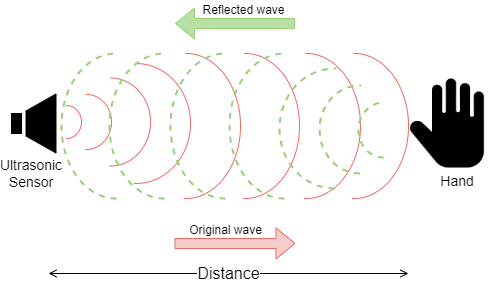
\includegraphics[width=0.7\textwidth]{img/Chap4/UltrasonicSensorFunction.png}
	\caption{Illustration of how the ultrasonic sensor works}
	\label{fig:Chap4-UltrasonicSensorFunction}
\end{figure}

\begin{wrapfigure}{r}{0.475\textwidth}
  \begin{center}
  	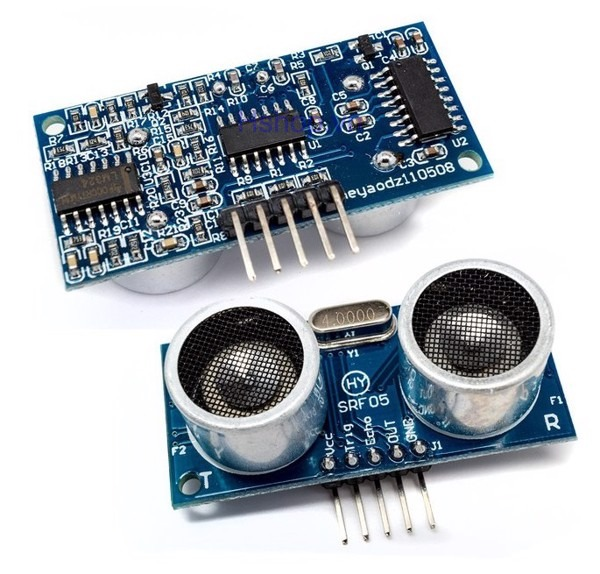
\includegraphics[width=0.3\textwidth]{img/Chap4/UltrasonicSensor.jpeg}
  \end{center}
	\caption{The ultrasonic sensor HY-SRF05}
  \label{fig:Chap4-UltrasonicSensorHYSRF05}
\end{wrapfigure}

In the thesis, we use the ultrasonic sensor HY-SRF05 (Figure \ref{fig:Chap4-UltrasonicSensorHYSRF05}), which is relatively inexpensive and meets our requirement for measuring the distance between the camera and the hand. According to the retailer, this sensor has a scanning range of up to 15 degrees. Furthermore, its scanning range is between 2 cm and 450 cm, with a relative error of around 0.3 cm. Furthermore, the most accurate measurement distance is less than 100 cm, which is more than enough to measure from the user's forehead to their waist.

However, the sensor method has yet to produce the desired result. The sensor can only detect one hand at a time, but what if sign language uses both hands at the same time? In this case, we cannot achieve the best possible results with only one sensor.

From there, we propose the following solution for measuring this distance. Replace the distance measurement method based on object size with one that uses a location sensor. It is similar to the zooming method, but it is superior in that it does not depend on the size of the hand, making it ideal for determining the distance for the problem we are attempting to solve.

This method is as follows. We will use the following formula:
\begin{center}
  $ distance\_predict = A*distance\_input + B*distance\_input + C $ 
\end{center}

In which $distance\_input$ will be the distance between two points (5,17) on the hand model taken from the MediaPipe model, and $distance\_predict$ will be the distance from the camera to the hand.

The trio of coefficients A, B, and C will be determined by interpolating the above polynomial with a pre-prepared data set. After having the above three coefficients, combined with calculating the distance between 2 points 5 and 17, we will quickly deduce the hand's distance. 

Figure \ref{fig:Chap4-LocationModule} shows the result we get

\begin{figure}[H]
	\centering
	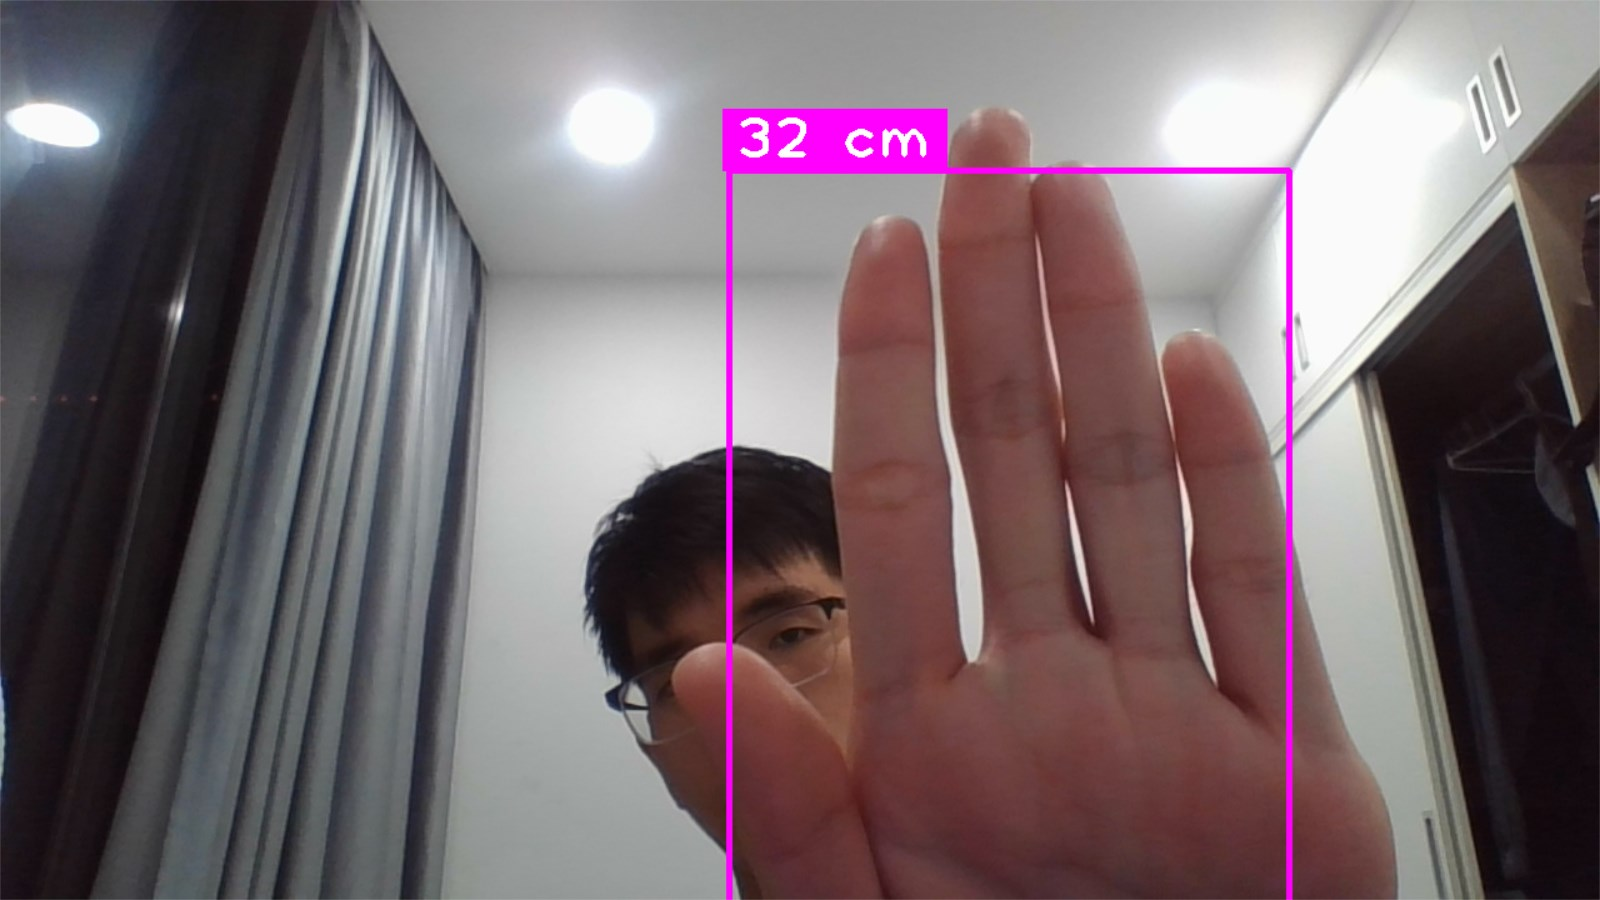
\includegraphics[width=0.7\textwidth]{img/Chap4/Location_00.jpg}
	\caption{Result of location module}
	\label{fig:Chap4-LocationModule}
\end{figure}

As a result, after receiving the result from this location module, we placed it in the hand state. Similarly, in the Section that follows, we will discuss how that hand state will aid us in translating sign language into Vietnamese.

% TODO
  % New approach : Sử dựng phương pháp khác để có thể đo khoảng cách
  % [ ] Thêm hình ảnh 
  % [ ] Giải thích
  
  % Thay thế phương pháp đo khoảng cách bằng sóng âm bằng phương pháp đo khoảng cách dựa trên hình ảnh 
  % Công thức: ...
  % Sử dụng phép nội suy đa thức để suy ra giá trị của các tham số A,B,C. 
  
  % Chúng ta sẽ tính khoảng cách giữa 2 điểm 5 và 17 trên bàn tay, sau đó sử dụng kết quả vừa tính toán được và công thức đã nêu ở trên để suy ra khoảng cách thực tế của bàn tay

  % Sau khi khoảng cách đã được ước lượng, ta sẽ suy ra được vị trí hiện tại của bàn tay đang ở đâu trên cơ thể (đầu, ngực hay bụng)

\subsection{Word decoder}
% TODO:   Previous approach 

% [x] How to map word ?

% TODO:   New approach

% [x] Punish function

% [x] Using beam search

% [x] CTC decode

% [x] Flow

% [x] Expected result

% [...] Difficult and proposed solution

% [...] Dịch sang tiếng anh

% [...] Thêm các hình ảnh


% TODO: With previous approach

As previously discussed, there are significant technical challenges in implementing the action detection module. We conducted research and proposed a new model to address these issues. As a result, this change has an impact on the word decoder module, which requires some tweaking.

The previous model breaks down a word into four components: pattern, location, direction, and action. It will search the database for the corresponding word after receiving the outputs from the four modules. Figure \ref{fig:Chap4-MapWord} demonstrates how a four-factor input is mapped to the correct word in the database. We have the system use a basic searching algorithm to find the most appropriate word. If none are found, it will replace or deprecate some parts of the input before attempting to find another word. The application will display the appropriate word on the screen after decoding it.

\begin{figure}[H]
	\centering
	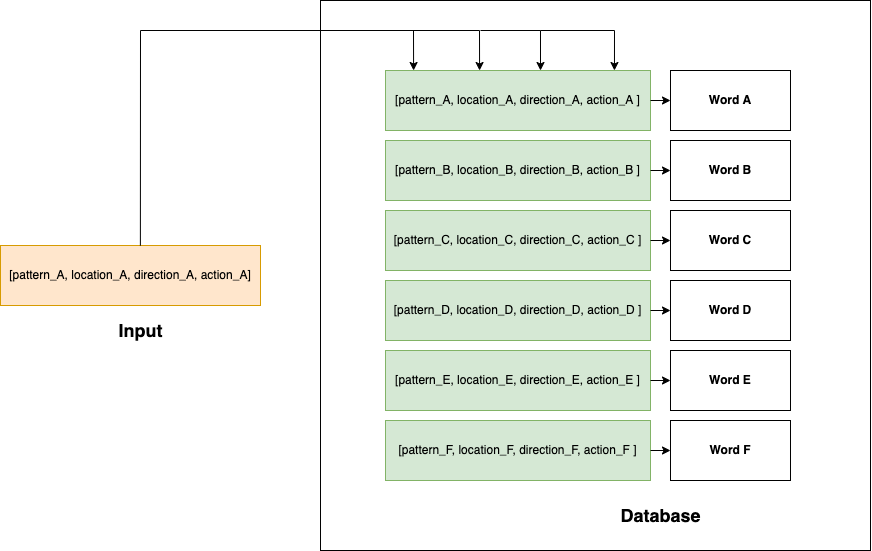
\includegraphics[width=\textwidth]{img/Chap4/MapWord.png}
	\caption{Map one to one data from four component with word in database and get result}
	\label{fig:Chap4-MapWord}
\end{figure}

\subsubsection{ Introduction to handstate }\label{sec:handstate}

The question that arises immediately following the deprecation of the action detection module is how we can find the correct word without that module. As a result, unlike the previous model, we propose a different model for a word that is not encoded into four factors. It only has three remaining elements: pattern, direction, and location. As a result, each combination of those three elements is referred to as a hand state (Figure \ref{fig:Chap4-HandState}), and a word can be decoded into a variety of hand states.

This concept of hand state stems from natural language processing research, in which a word is made up of many characters. As a result, a word is concatenated from several hand states in the thesis. Then, after going through the processing steps discussed later in this proposal, we will get the desired word.

\begin{figure}[H]
  \centering
  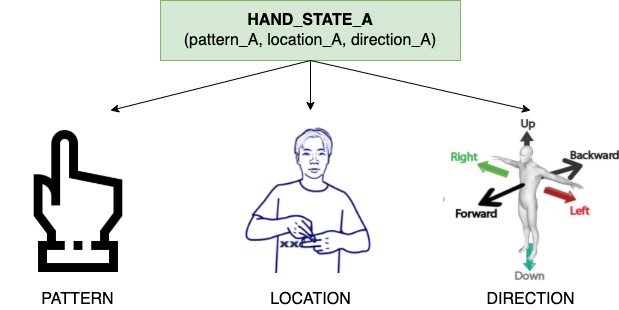
\includegraphics[width=0.6\textwidth]{img/Chap4/HandState.png}
  \caption{ Hand state which construct from pattern, location and direction}
  \label{fig:Chap4-HandState}
\end{figure}

\subsubsection{ Using beam search and CTC decode to map word}

After we have grasped the concept of hand state, we will proceed to the most important part of the model: converting the received hand states into words.      

\begin{figure}[H]
  \centering
  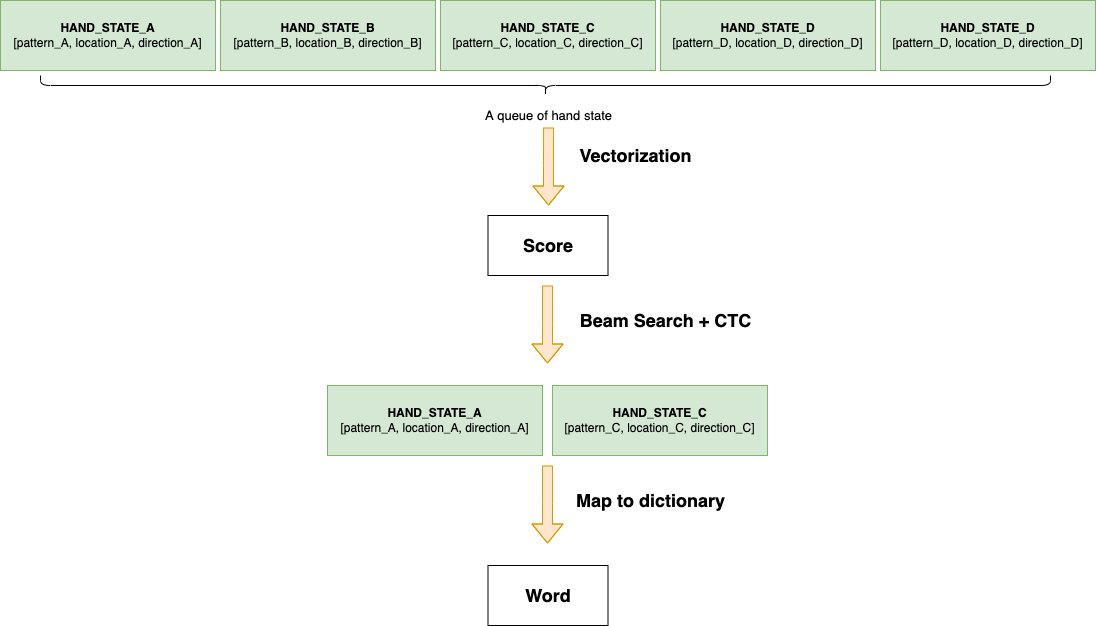
\includegraphics[width=\textwidth]{img/Chap4/Architechture.png}
  \caption{Architecture}
  \label{fig:Chap4-Architechture}
\end{figure}

The authors' model for this Section is shown in Figure \ref{fig:Chap4-Architechture}. A queue of hand states from the previous three components will be used as input. The queue length is set to 5 in our conventions, but this is not the final number because we need more calculations and experimentation to find the optimal queue length. This model is comprised of three steps:

\begin{enumerate}
  \item \textbf{Vectorization:} This step converts a queue of many hand states (Figure \ref{fig:Chap4-HandStateQueue}) into a matrix for beam search input.
  \item \textbf{Beam search:} In this step, we will use a beam search algorithm to determine which hand states are appropriate for the database input. Furthermore, we propose using the CTC decode model to eliminate incorrect or previously duplicated hand states, increasing the model's efficiency.
  \item \textbf{Map to the dictionary:} Finally, after going through the preceding two steps, we will obtain the most likely hand state from the initial queue. Our job is to match these hand states to the correct word in the database.
\end{enumerate}
      
\subsubsection{ Vectorization }
% TODO: Why we need punish
% TODO: how to perform -> Trình bày cách đánh giá như thế nào, cách trừ điểm và các phương châm đánh giá
% TODO: Sau khi punish dùng hàm softmax để chuyển các giá trị về dạng xác suất

We get a list of hand states when we get to this step. Because we need a matrix representing the correlation between the component outputs and the data in the database before entering the beam search module.

\begin{figure}[H]
  \centering
  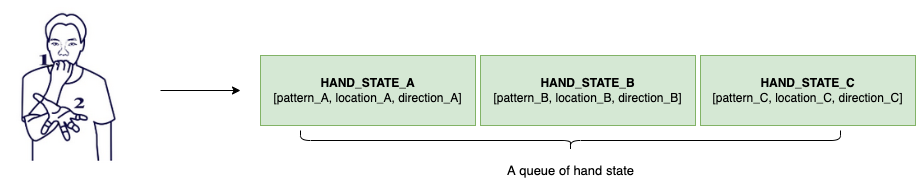
\includegraphics[width=\textwidth]{img/Chap4/HandStateQueue.png}
  \caption{A queue of hand states to sign "Thank you"}
  \label{fig:Chap4-HandStateQueue}
\end{figure}

From this queue, we will cycle through each hand state, compare it to the available hand state database, and calculate the score based on the principles shown in Figure \ref{fig:Chap4-Vectorization}:

\begin{enumerate}
  \item If the word in the hand matches the word in the database, the score will be increased.
  \item Otherwise, if that hand state does not match any, the score will be reduced.
\end{enumerate}

\begin{figure}[H]
  \centering
  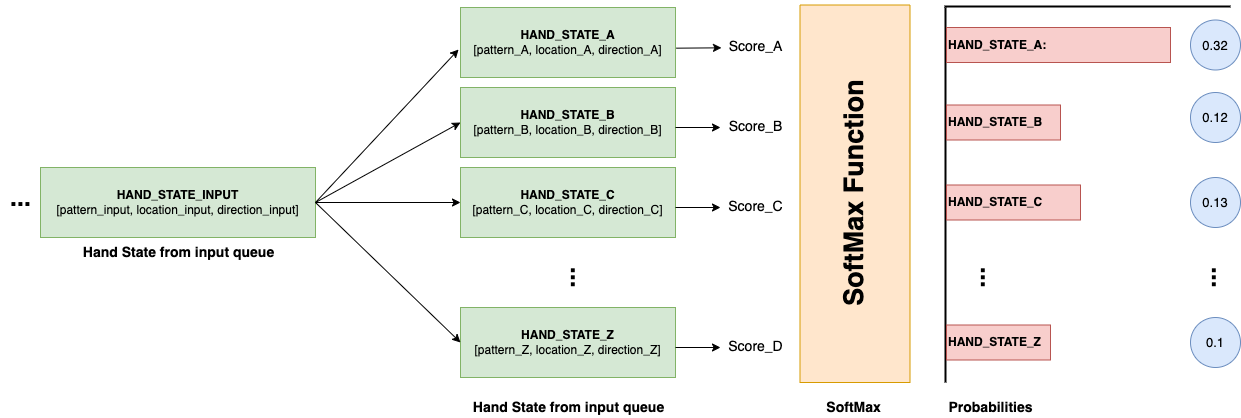
\includegraphics[width=\textwidth]{img/Chap4/Vectorization.png}
  \caption{ Vectorization }
  \label{fig:Chap4-Vectorization}
\end{figure}
% TODO: Change to Math

The first principle states that the higher the score, the more similar the hand state retrieved from the queue is to that in the database. For example, in the database, we have the following hand state:

$\begin{bmatrix}
  pattern \_ A & location \_ A & direction \_ A
\end{bmatrix}$
, and the hand state we get from the input is 
$\begin{bmatrix}
  pattern \_ A & location \_ A & direction \_ A
\end{bmatrix}$
then this hand state will be rated higher than the hand state 
$\begin{bmatrix}
  pattern \_ A & location \_ A & direction \_ B
\end{bmatrix}$
. And so forth. In turn, we will score the hand states taken from the queue.

The minus point is evaluated on the second point based on its matching pattern with the hand states in the database. When the system recognizes patterns from the hand pattern recognition module (via the vision approach), they are likely to be incorrectly detected. We devised a rule to address this issue and improve the accuracy of the results. The minus point will be lower for patterns that are difficult to detect than for simple ones. In short, the smaller the minus point, the more complex the pattern to be recognized.

% + Khi đánh giá các hand state, đối với trường hợp so trùng 2 pattern. Do các pattern này được nhận diện từ module hand pattern regconition (vision approach), do đó, sẽ có khả năng bị nhận diện bị sai, hoặc bị nhầm. Vì lẽ đó, để có thể đánh giá một cách chính xác và công bằng nhất có thể thì ở đây, đối với những pattern hay bị nhận diện sai, ta sẽ trừ điểm thấp và ngược lại, với những pattern đơn giản mà hệ thống lại nhận diện sai thì sẽ bị trừ điểm nhiều hơn.

Following the completion of the preceding evaluation and scoring steps, we will use a function to normalize the data (here, the authors use the softmax function\cite{SoftMax}) and return a set of probabilities for the hand states in the row. Wait. This set of probabilities will be used as input for the beam search step.

\subsubsection{ Using beamsearch with CTC decode }
% TODO: Trình bày cách sử dụng beamsearch để tìm các cặp bộ 3
% TODO: Image beamsearch (get from ppt)
% TODO: Example
% TODO: Áp dụng CTC để handle một số trường hợp
% TODO: Các khó khăn gặp phải và hướng giải quyết

The hand states in our queue have been converted to a MxN matrix after passing the vectorization step, where M is the length of the hand state's database and N is the length of the queue.

We will retrieve the most likely k-hand state from the database by using beam search (Figure \ref{fig:Chap4-BeamSearch}). We can imagine what happened later during the beam search based on the image below.

% Sau khi qua bước vectorizaion, các hand state trong hàng đợi của chúng ta
% đã được chuyển đổi thành một ma trận MxN với M là độ dài của cơ sở dữ liệu về
% các hand state và N là độ dài của hàng đợi.
      
% Bằng việc sử dụng beam search, từ sẽ thu được k hand state có khả năng nhất
% từ cơ sở dữ liệu. Từ hình ảnh bên dưới, ta có thể hình dung được những gì
% đã diễn ra sau trong quá trình thực hiện beam search

% FIXME: Insert image from ppt about matrix with beam search

\begin{figure}[H]
  \centering
  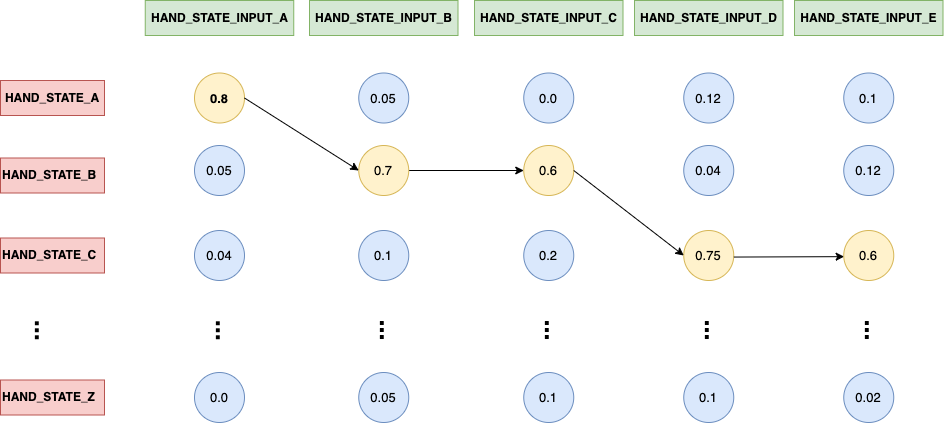
\includegraphics[width=\textwidth]{img/Chap4/BeamSearch.png}
  \caption{ Beam Search }
  \label{fig:Chap4-BeamSearch}
\end{figure}

However, as we can see, after the beam search step, we will get a sequence of hand states with a length equal to the length of the input queue. These hand states may contain duplicate hand states or incorrect hand states. As a result, we must use the CTC algorithm to remove the hand states from infection. We will set a threshold in the vectorization step to discard these hand states and treat them as a blank character for the incorrect hand states. Furthermore, we will get the desired result after beam search CTC decode.

% Tuy nhiên, có thể thấy được rằng, sau khi thực hiện xong bước beamsearch,
% ta sẽ thu được một dãy các hand state có độ dài tương ứng với độ dài của hàng đợi
% , các hand state này có thể bao gồm những hand state bị trùng nhau, hoặc cũng có thể
% là những hand state bị sai. Do đó, ta cần áp dụng thêm CTC decode để loại bỏ các hand state
% bị trùng này. Đối với những hand state bị nhận sai từ những module trước thì ở bước Vectorization,
% ta sẽ đặt một threshold để loại bỏ những hand state này và xem như hand state đó là một ký tự rỗng (" ")
% và cuối cùng, sau khi áp dụng CTC decode vào, ta sẽ thu được kết quả mong muốn

% FIXME: Insert image about the result (get from ppt)

      
      
    \subsubsection{ Map to dictionary }
      % TODO: Cách map như thế nào

      \begin{figure}[H]
        \centering
        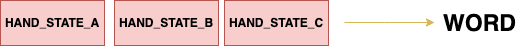
\includegraphics[width=\textwidth]{img/Chap4/Result.png}
        \caption{ Map to dictionary and get word }
        \label{fig:Chap4-Result}
      \end{figure}

      % Sau khi nhận được một tập các hand state có khả năng nhất, việc còn lại là
      % chúng ta sẽ map vào cơ sở dữ liệu, như cách mà chúng ta đã làm trong mục ..., 
      % nhưng thay vì map với bộ 4 thành phần thì ở đây, ta sẽ map với input các hand state thu được
      % từ bước ... .
      % Và như thế, ta sẽ thu được từ vựng mà không cần phải dùng tới module action detection.

All that remains is for us to map to the database, as we did in the previous Section, but instead of mapping with a 4-component set, we will map with input retrieved from this previous step. Finally, without using the action detect module, we will obtain the word (Figure \ref{fig:Chap4-Result}).

\subsection{Text-to-Speech}

Furthermore, because people do not always read the result from the phone's screen, the application can speak it out loud to make it easier for them to know the answer after the translation process. One method is to create a database of many sound files that have been tagged with the corresponding Vietnamese word. This approach, however, is inefficient because it necessitates a significant amount of effort to create the database. Every single word must be recorded and then mapped together.

Instead, we apply a well-known speech service from Google known as Text-to-Speech\cite{GG:Text-to-Speech}. Text-to-Speech, according to Google, converts text input into natural human speech audio data. Furthermore, this service supports a wide range of languages, including the one we require, Vietnamese. Using the API provided by that speech service, our application can speak up the result without requiring a large sound database on the user's phone.

This API is available for free. The cost of text-to-speech is determined by the number of characters sent to the service each month to be synthesized into audio. According to Google, "the first 1 million characters for WaveNet voices are free each month." Each month, the first 4 million characters for standard (non-WaveNet) voices are free. After the free tier, Text-to-Speech is charged per 1 million text characters processed. The thesis only requires the standard (non-WaveNet) plan, which includes 4 million characters for free each month and costs USD 4.00 for each additional 1 million characters. The number of characters we will use in the upcoming phases of building the application is negligible in comparison to the 4 million free characters. As a result, we decided to use the Google service to implement this Text-to-Speech module.

\subsection{The camera module}

After discussing the solutions and implementations of the system's soft modules, we must move on to the main one, which is considered the thesis's eyes, which is the camera module. This Section will go over the components of a camera module and show some images of a real one that we built.

Parts for the camera modules are easily available from any retailer that sells electrical components, robots, and Arduino kits. Furthermore, in this day and age of e-commerce, it is much easier to find and compare the components that we require online. The components needed to construct a camera module are listed below.

First, we require a camera component, which the ESP32-CAM is ideal for. It is inexpensive and simple to use, which makes it ideal for our thesis, which requires complex functions such as image tracking and recognition. Furthermore, it incorporates Wi-Fi and traditional Bluetooth, allowing us to send images to the user's smartphone for the next steps in sign language translation.

Second, we will require a converter adapter to assist us in sideloading the program into the camera module. The ultrasonic sensor mentioned in the Section \ref{sec:locationDetection} is the third component we require. It aids in location detection by informing the system of the distance between the hands and the camera module. Last but not least, this camera module requires a battery to power the entire module, and we believe that a volume of around 100 mAh is adequate.

Furthermore, all of the above components must be stored in a box. We designed that package on Tinkercad, an online 3D modeling program that runs in a web browser, using current 3D printing technology. After gathering all of the necessary components, we attempted to put them together and obtained the result shown below.

\begin{figure}[H]
	\centering
	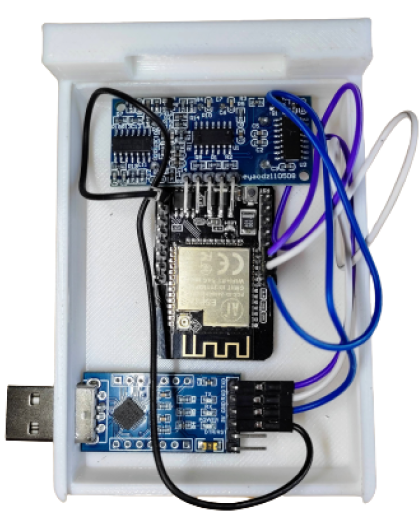
\includegraphics[width=0.45\textwidth]{img/Chap5/Prototype_View_inside.png}
	\caption{The components inside the camera module prototype}
\end{figure}

\begin{figure}[H]
	\centering
	\begin{subfigure}[b]{0.45\textwidth}
		\centering
		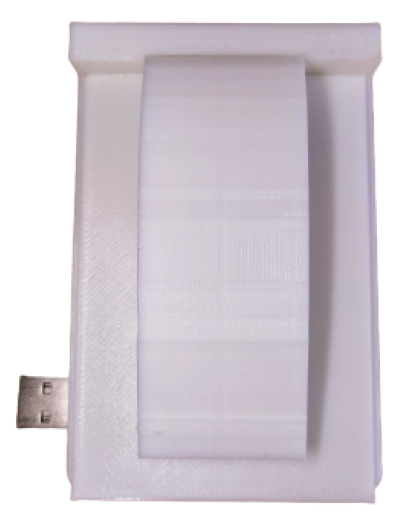
\includegraphics[width=\textwidth]{img/Chap5/Prototype_View_above.png}
	\end{subfigure}
	\hfill
	\begin{subfigure}[b]{0.46\textwidth}
		\centering
		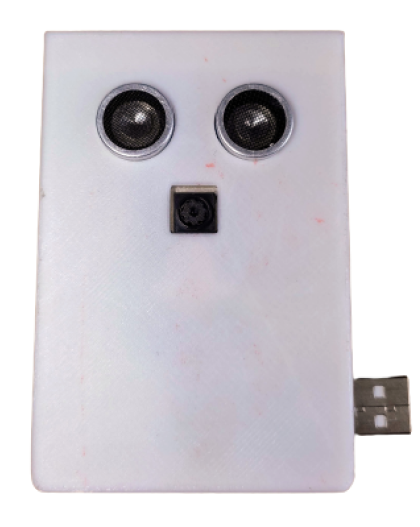
\includegraphics[width=\textwidth]{img/Chap5/Prototype_View_under.png}
	\end{subfigure}
	\caption{Views of the camera module prototype from the above and under}
\end{figure}

\begin{figure}[H]
	\centering
	\begin{subfigure}[b]{0.45\textwidth}
		\centering
		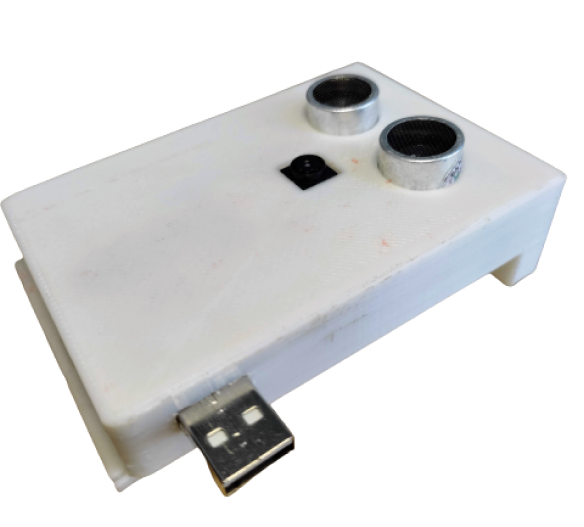
\includegraphics[width=\textwidth]{img/Chap5/Prototype_View_side_1.png}
	\end{subfigure}
	\hfill
	\begin{subfigure}[b]{0.45\textwidth}
		\centering
		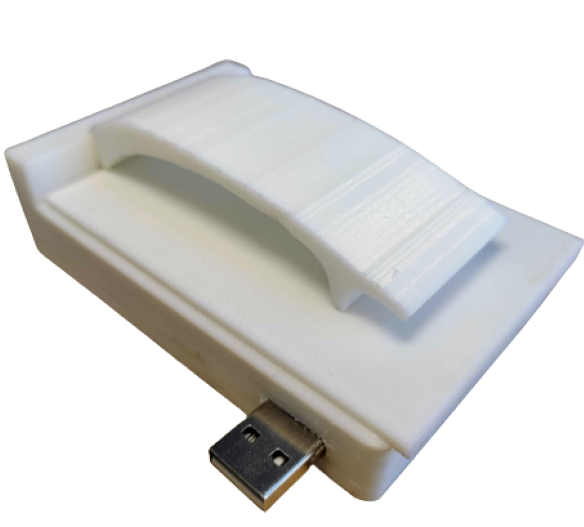
\includegraphics[width=\textwidth]{img/Chap5/Prototype_View_side_2.png}
	\end{subfigure}
	\caption{Views of the camera module prototype from the sides}
\end{figure}

Nonetheless, the box's cover is difficult to insert due to the smallest number that a 3D printer can print. The hanger that assisted in hanging the box on the hat is not as flexible as we had hoped, so it needs to be redesigned.

\subsection{App design}

The application must meet user experience and user interface requirements. And, as part of the thesis research, we created a prototype for the application, which included one additional feature in addition to the main one. A sign language dictionary is one of the extra features. Table \ref{tab:4-dictionary} demonstrates this feature.

Before delving into the design of this application, it is important to note that they do not yet cover all of the screens required for the application. And they do not represent the final design that we have. However, when designing this prototype, we followed some conventions, such as rounding the corners and keeping the colors pale and not too bright, in order to make the users feel calm and at ease while using the application.

\begin{figure}[H]
	\centering
	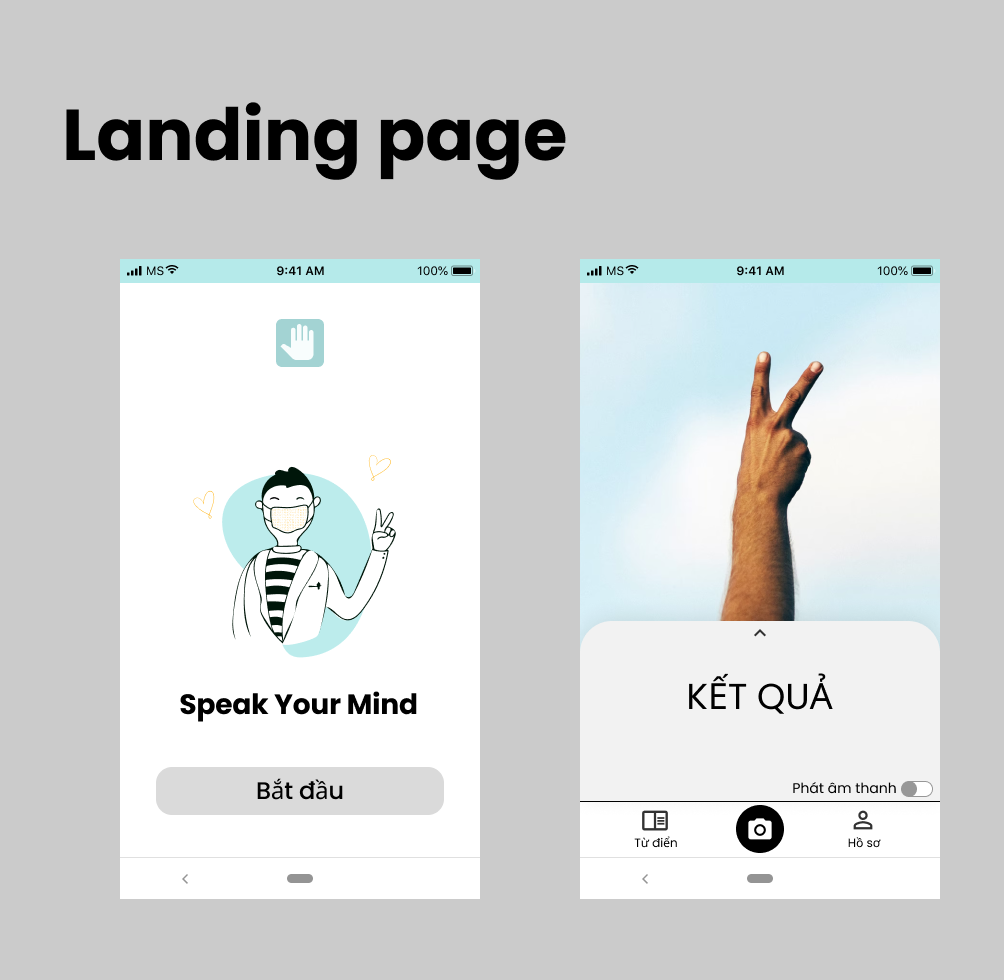
\includegraphics[width=0.8\textwidth]{img/Chap5/Landing_page.png}
	\caption{The landing page of the application}
\end{figure}

\begin{figure}[H]
	\centering
	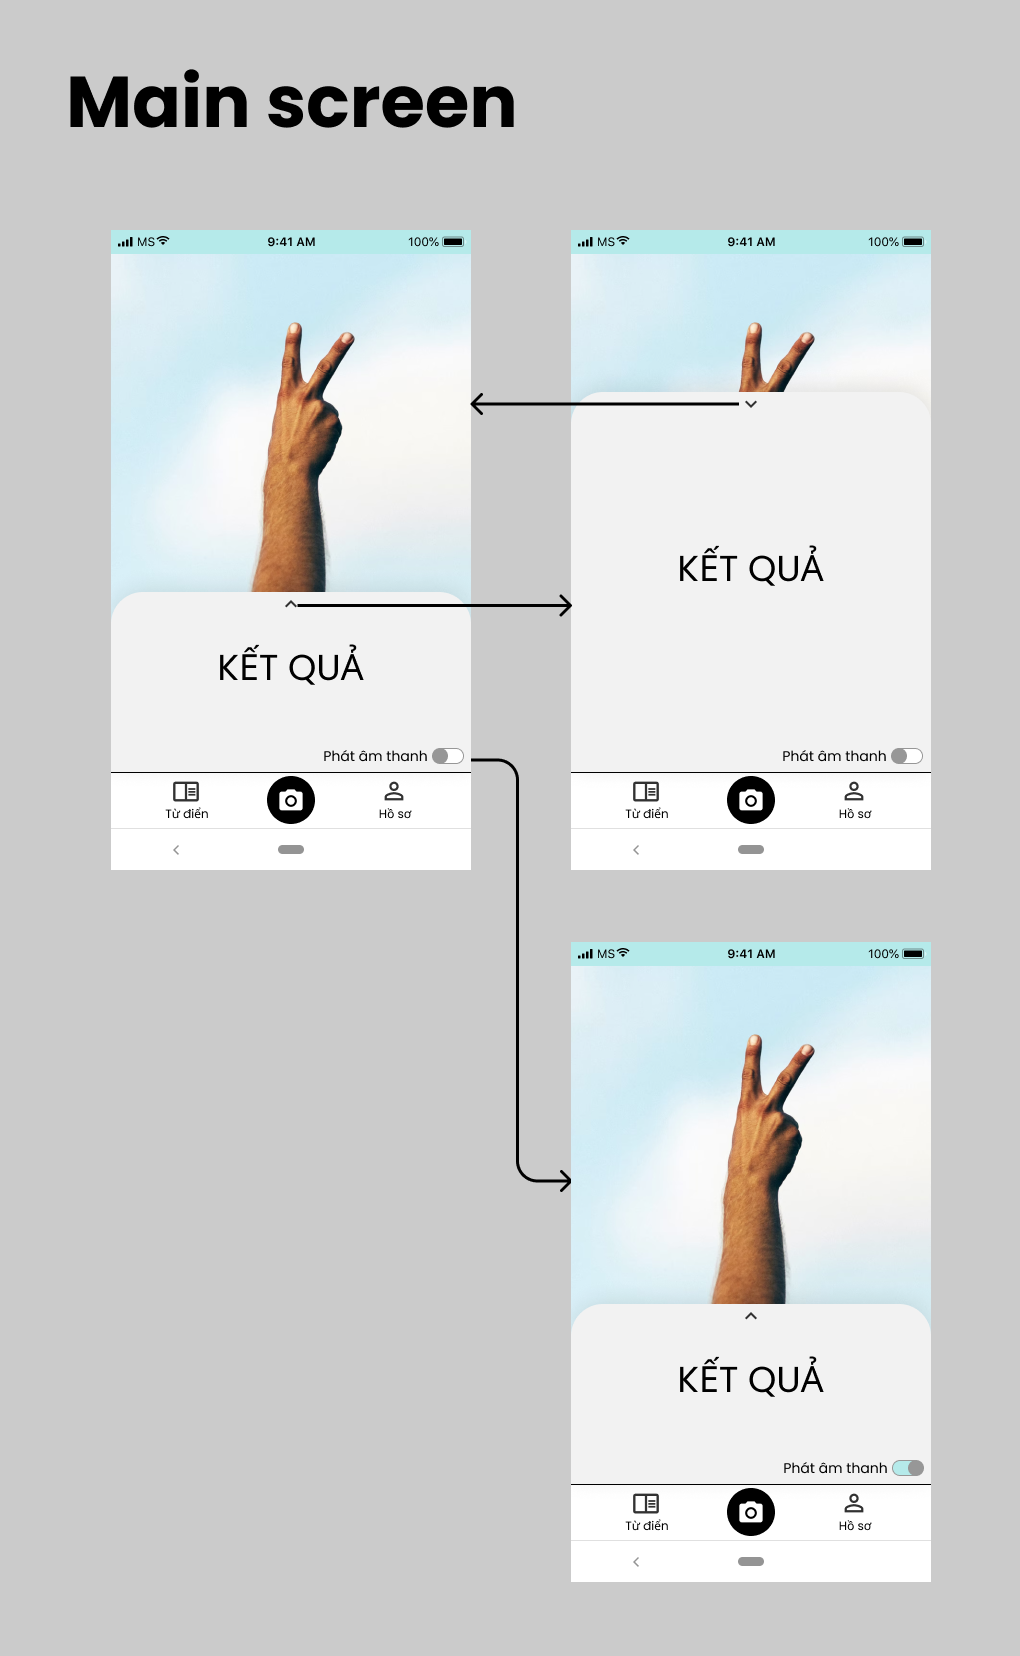
\includegraphics[height=0.8\textheight]{img/Chap5/Main_screen.png}
	\caption{The main screen of the application}
\end{figure}

% \begin{figure}[H]
% 	\centering
% 	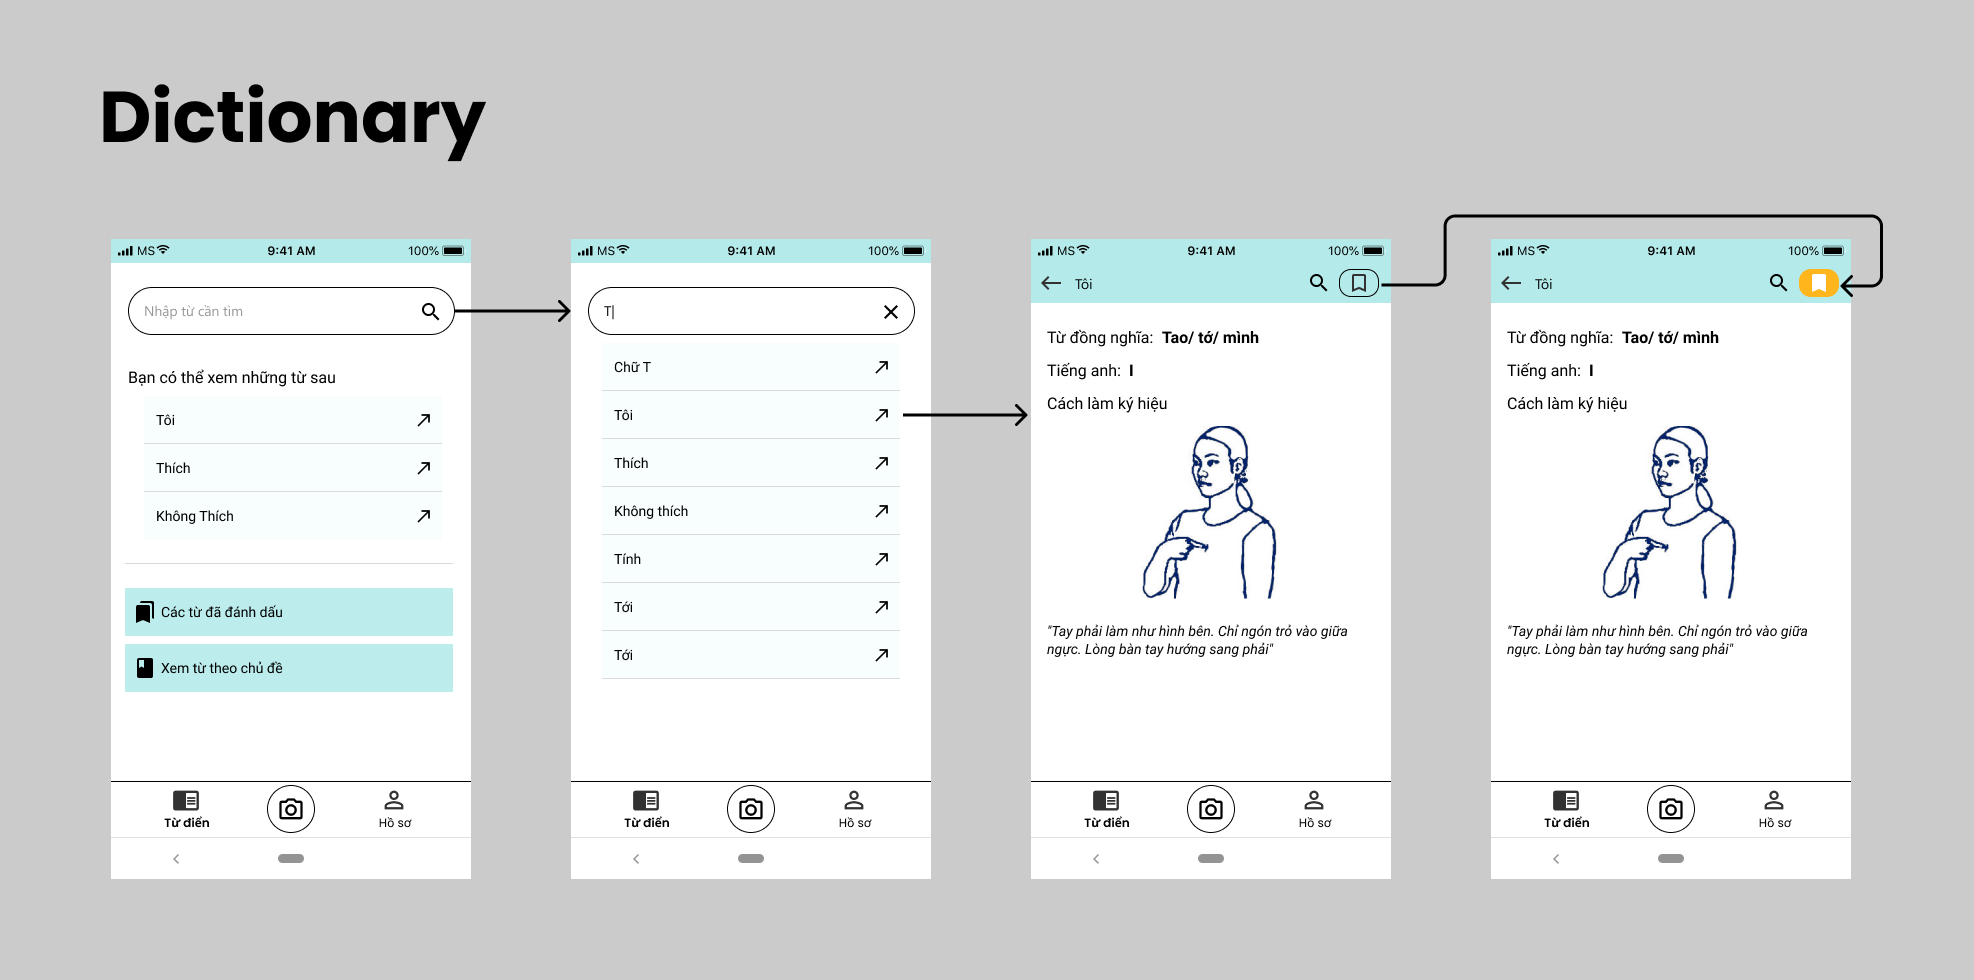
\includegraphics[width=\textwidth]{img/Chap5/Dictionary.png}
% 	\caption{The main screen of the application}
% \end{figure}

\begin{figure}[H]
	\centering
	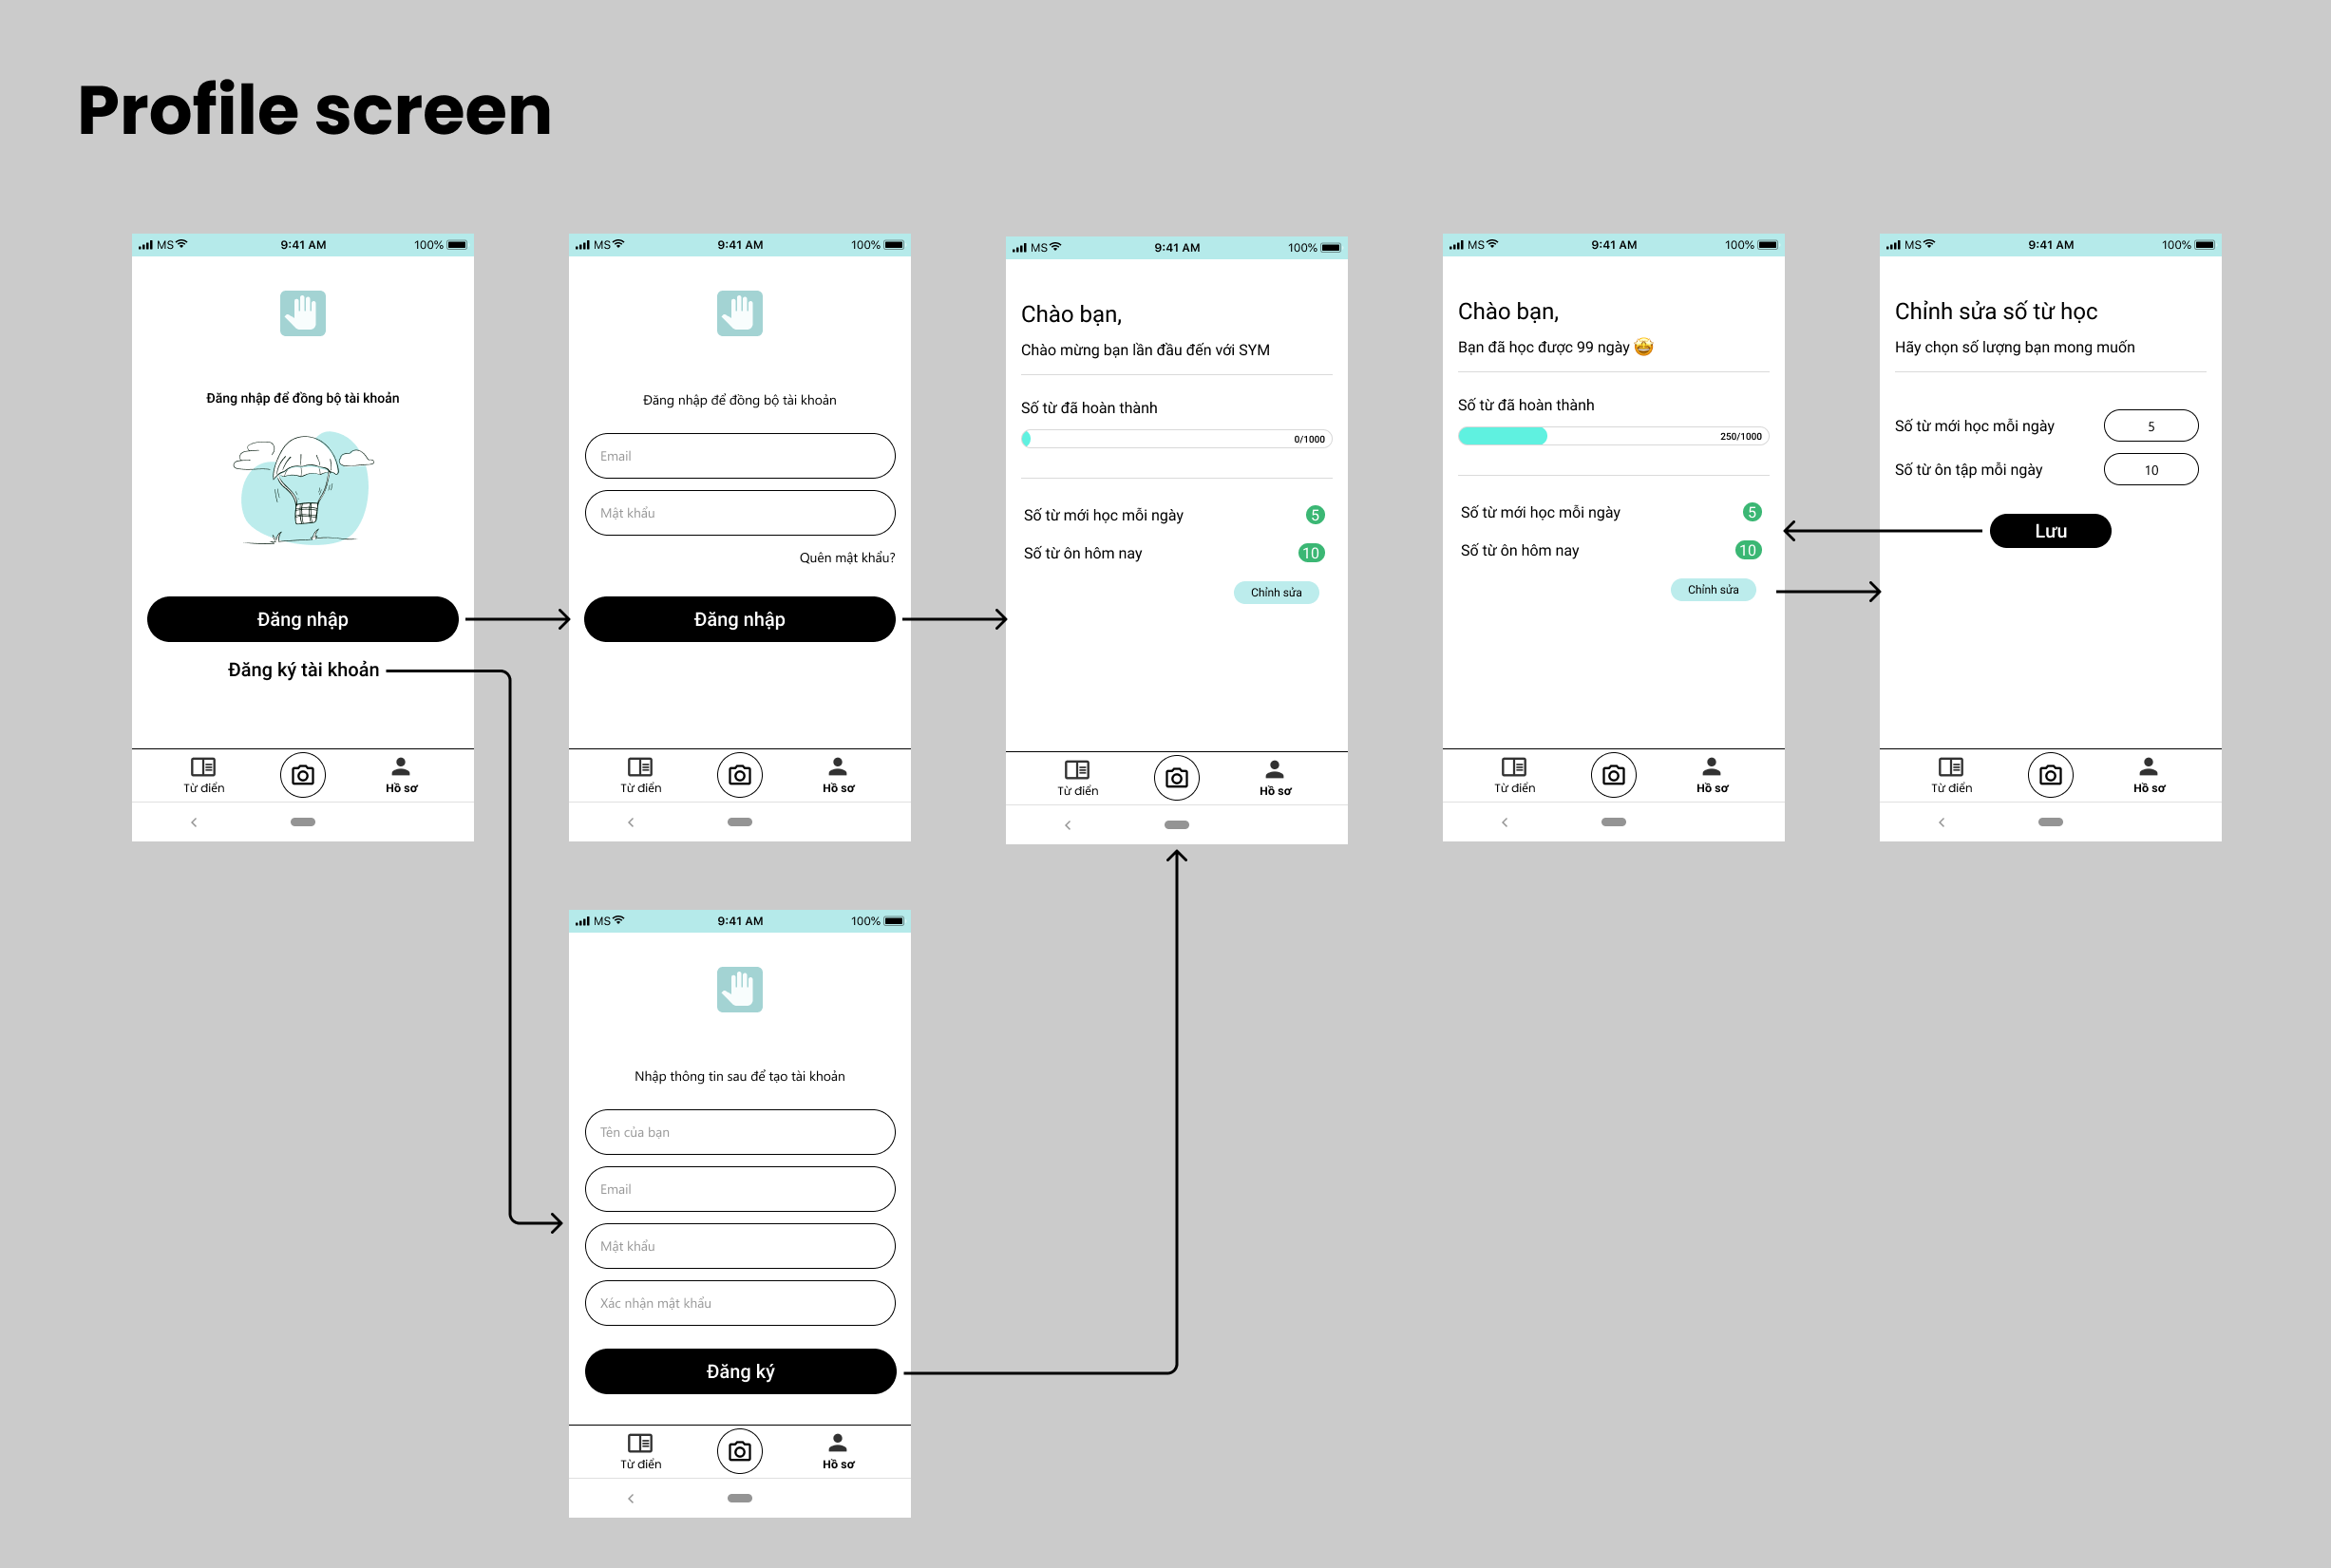
\includegraphics[width=\textwidth]{img/Chap5/Profile_screen.png}
	\caption{The profile screen}
\end{figure}

\begin{figure}[H]
	\centering
	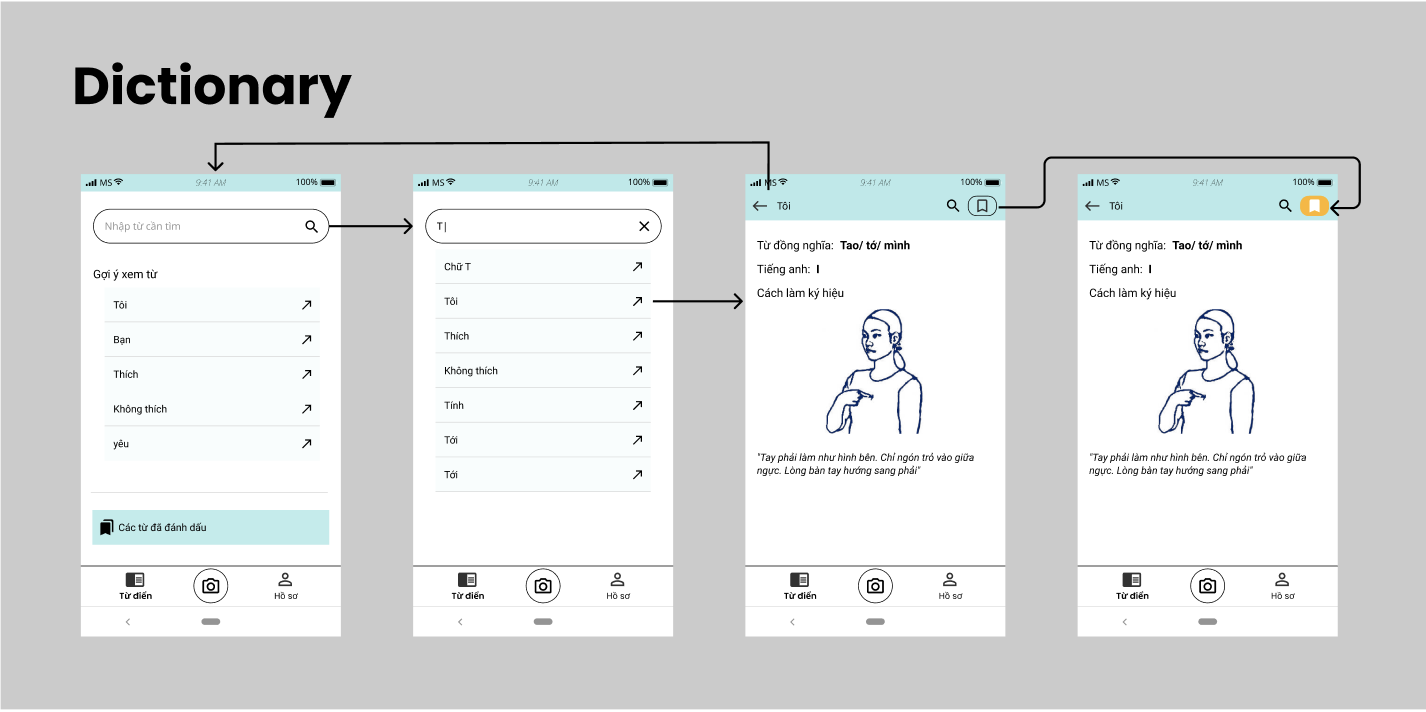
\includegraphics[width=\textwidth]{img/Chap4/Dictionary.png}
	\caption{The dictionary screen}
\end{figure}


% Vẽ use-case
% [ ] Use-case 
%   + Xem kết quả từ được trả về sau khi dự đoán
%   + Đăng nhập/ Đăng xuất
%   + Đăng ký
%   + Xem profile
%   + Xem từ điển


% [ ] Use-case description     

\newpage
\subsection{Use case}

On the whole, Figure \ref{fig:Chap4-usecase} illustrates the project's overall use-case.

\begin{figure}[H]
	\centering
	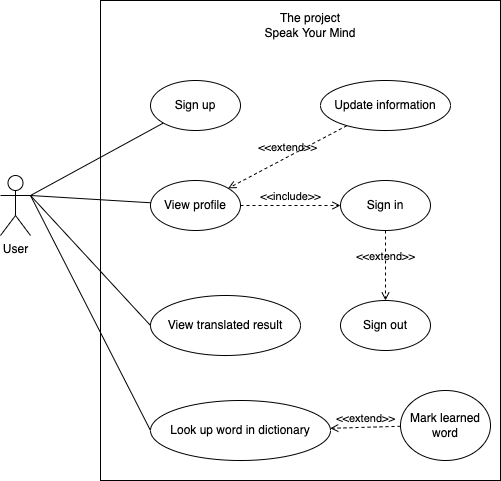
\includegraphics[width=\textwidth]{img/Chap4/use-case.drawio.png}
	\caption{Use case diagram}
  \label{fig:Chap4-usecase}
\end{figure}

\subsection{Use case description}

\subsubsection{View translated result}
\begin{table}[H]
  \centering
  \begin{tabular}{ |l| p{11cm}|}
    \hline
    Use case ID & 1 \\ 
    \hline
    Use case name & View translated result \\ 
    \hline
        Description & The user is informed about the hand gesture he just made\\
        \hline
        Actor & User\\
        \hline
        Post-condition(s) & Successful sign language detection and return to the user\\
        \hline
        \multirow{4}*{Normal flow}  & 1. The user visits the main page\\
        						        & 2. The user signs the word\\
        					            & 3. Application that records actions and makes predictions\\
        					            & 4. The application displays the result after translated successfully\\
        \hline
        \multirow{3}*{Exception flow}   & Exception1: \\
                                            & 4a. The application cannot translate the sign language\\
                                            & 5a. The application shows no more information and ends\\
        \hline
  \end{tabular}
  \caption{Use case view translated result}
\end{table}



% Chỉnh sửa lại phần này, thêm alternative flow về việc chỉnh sửa profile
\subsubsection{View profile}
\begin{table}[H]
  \centering
  \begin{tabular}{ |l| p{11cm}|}
    \hline
    Use case ID & 2 \\ 
    \hline
    Use case name & View profile \\ 
    \hline
        Description & The user can view his personal information and edit the number of learned words and the number of new words learned in the day\\
        \hline
        Actor & User\\
        \hline
        Post-condition(s) & The user sees his information page\\
        \hline
        \multirow{3}*{Normal flow}  & 1. User visits the profile page \\
        						        & 2. The application connects to the system in order to obtain information about the user\\
        					            & 3. The application displays user data\\

        \hline
        Alternative flow & Null \\ 
        \hline
        Exception flow   & Null \\
        \hline
  \end{tabular}
  \caption{Use case view profile}
\end{table}

\subsubsection{Sign up}
\begin{table}[H]
  \centering
  \begin{tabular}{ |l| p{11cm}|}
    \hline
    Use case ID & 3 \\ 
    \hline
    Use case name & Sign up \\ 
    \hline
        Description & The user must first create a personal account to access the system\\
        \hline
        Actor & User\\
        \hline
        Pre-condition(s) & The device must be connected to the internet\\
        \hline
        Post-condition(s) & Successful account registration\\
        \hline
        \multirow{5}*{Normal flow}  & 1. The user taps on “Đăng ký tài khoản” button \\
        						        & 2. The application displays the account registration view\\
                            & 3. The user enters the necessary data\\
                            & 4. The user taps the "Đăng ký" button \\
                            & 5. The application redirect the user to the login screen\\
        \hline
        \multirow{4}*{Alternative flow}   & A. The user abandons the account creation process and wishes to return to the login screen\\
                                          & 3.1 The user taps the "Đăng nhập” button and the application jumps to step 5 \\
        \hline
        Exception flow   & If there is no internet connection, the application displays the message "Không có kết nối mạng, vui lòng thử lại sau." \\
        \hline
  \end{tabular}
  \caption{Use case sign up}
\end{table}

\subsubsection{Sign in}
\begin{table}[H]
  \centering
  \begin{tabular}{ |l| p{11cm}|}
    \hline
    Use case ID & 4 \\ 
    \hline
    Use case name & Sign in \\ 
    \hline
        Description & Allow the user to sign in to his account in order to use the application's services\\
        \hline
        Actor & User\\
        \hline
        Pre-condition(s) & The device must be connected to the internet\\
        \hline
        Post-condition(s) & The user successfully logs in.\\
        \hline
        \multirow{4}*{Normal flow}  & 1. The application displays the login page\\
        						        & 2. The user enters his email address and password in the appropriate fields.\\
        					            & 3. The user taps the "Đăng nhập" button\\
                              & 4. The application shows “Logged in successfully” \\ 
                              & 4. The application direct the user to the main screen\\ 
        \hline
        \multirow{12}* {Alternative flow}  & A. The user enters wrong email address\\
                                          & 4.1 The application shows "Email không tồn tại" \\ 
                                          & 4.2 Application goes back to step 2 \\ 
                                          & B. The user enters invalid email address
                                          4.1 The application shows "Email không đúng định dang" \\ 
                                          & 4.2 Application goes back to step 2 \\ 
                                          & C. The user enters wrong password\\
                                          & 4.1 The application shows “Mật khẩu không đúng” \\ 
                                          & 4.2 Application goes back to step 2\\
        \hline
        Exception flow   & If there is no internet connection, the application displays the message "Không có kết nối mạng, vui lòng thử lại sau." \\
        \hline
  \end{tabular}
  \caption{Use case sign in}
\end{table}


\subsubsection{Sign out}
\begin{table}[H]
  \centering
  \begin{tabular}{ |l| p{11cm}|}
    \hline
    Use case ID & 5 \\ 
    \hline
    Use case name & Sign out \\ 
    \hline
        Description & The user wants to sign out the current account\\
        \hline
        Actor & User\\
        \hline
        \multirow{2}*{Pre-condition(s)} & The device must be connected to the internet \\
                                        & The user logged in successfully \\ 
        \hline
        Post-condition(s) & The user signs out successfully\\
        \hline
        \multirow{2}*{Normal flow}  & 1. The user taps the "Đăng xuất" button \\
        						        & 2. The application returns to the login screen\\
        \hline
        Alternative flow  & No \\
        \hline
        Exception flow   & If there is no internet connection, the application displays the message "Không có kết nối mạng, vui lòng thử lại sau." \\
        \hline
  \end{tabular}
  \caption{Use case sign out}
\end{table}

\subsubsection{Look up word in dictionary}
\begin{table}[H]
  \centering
  \begin{tabular}{ |l| p{11cm}|}
    \hline
    Use case ID & 6 \\ 
    \hline
    Use case name & Look up word in dictionary \\ 
    \hline
        Description & The user needs to look up a word in the sign language dictionary\\
        \hline
        Actor & User\\
        \hline
        \multirow{1}*{Pre-condition(s)} & For the better result, the device should have internet connection \\
        \hline
        Post-condition(s) & The user successfully finds out how to sign the word\\
        \hline
        \multirow{2}*{Normal flow}  & 1. The user taps dictionary in the navbar\\
        						        & 2. The application directs the user to screen dictionary\\
        						        & 3. The user inputs the word and taps it on screen\\
        						        & 4. The application displays the word's corresponding information and includes an instructional video.\\
        \hline
        Alternative flow  & No \\
        \hline
        Exception flow   & If there is no internet connection, the application only shows the local information, and the video is note included. \\
        \hline
  \end{tabular}
  \caption{Use case look up word in dictionary}
  \label{tab:4-dictionary}
\end{table}

\subsubsection{Mark learned word}
\begin{table}[H]
  \centering
  \begin{tabular}{ |l| p{11cm}|}
    \hline
    Use case ID & 7 \\ 
    \hline
    Use case name & Mark learned word \\ 
    \hline
        Description & The user wishes to mark a word as learned in order to easily find it in the future.\\
        \hline
        Actor & User\\
        \hline
        \multirow{1}*{Pre-condition(s)} & Previously logged in \\ 
        \hline
        Post-condition(s) & The user marked the word, which increased the learning bar on the profile page\\
        \hline
        \multirow{2}*{Normal flow}  & 1. The user taps dictionary in the navbar\\
        						        & 2. The application directs the user to screen dictionary\\
        						        & 3. The user inputs the word and taps it on screen\\
        						        & 4. The application shows the corresponding information of the word, includes the instruction video\\
        						        & 5. User taps on the bookmark button on the top right\\
        						        & 6. That bookmark will change from outline state to filled state\\
        \hline
        Alternative flow  & No\\
        \hline
        Exception flow   & If the user hasn't logged in, the application will notify that "You have to login to perform this"\\
        \hline
  \end{tabular}
  \caption{Mark learned word}
  \label{tab:4-mark-learned-word}
\end{table}